\documentclass[12pt, letterpaper]{report}

% === PAQUETES BASE ===
\usepackage[utf8]{inputenc}
\usepackage[spanish]{babel}
\usepackage[left=3cm, right=2.5cm, top=2.5cm, bottom=2.5cm]{geometry}
\usepackage{graphicx}
\usepackage{setspace}
\usepackage{float}
\usepackage{csquotes}
\usepackage{array}
\usepackage{booktabs}
\usepackage{tabularx}
\usepackage{longtable}
\usepackage{multirow}
\usepackage[table,xcdraw]{xcolor}

% === TIKZ ===
\usepackage{tikz}
\usetikzlibrary{shapes.geometric, arrows, positioning, fit, backgrounds, shadows, calc, babel}

% === FUENTE ARIAL (Helvetica) ===
\usepackage{helvet}
\renewcommand{\familydefault}{\sfdefault}
\usepackage[T1]{fontenc}

% === BIBLIOGRAFIA APA 7 ===
\usepackage[style=apa, backend=biber]{biblatex}
\addbibresource{referencias.bib}

% === SIN SANGRIA ===
\usepackage[skip=10pt plus1pt]{parskip}
\setlength{\parindent}{0pt}
\onehalfspacing

% === ENCABEZADOS ===
\usepackage{fancyhdr}
\setlength{\headheight}{15pt}
\pagestyle{fancy}
\fancyhf{}
\fancyhead[L]{\nouppercase{\rightmark}}
\fancyhead[R]{\thepage}
\renewcommand{\headrulewidth}{0.5pt}
\renewcommand{\sectionmark}[1]{\markright{\thesection\ #1}}
\renewcommand{\chaptermark}[1]{\markboth{\thechapter\ #1}{}}

% === FORMATO DE TITULOS ===
\usepackage{titlesec}
\titleformat{\chapter}[display]
  {\bfseries\huge}
  {\raggedright\MakeUppercase{\chaptertitlename} \thechapter}
  {0.5ex}
  {\titlerule\vspace{1ex}\raggedleft}
  [\vspace{2ex}]
\titleformat{\section}{\normalfont\Large\bfseries}{\thesection.}{1em}{}
\titleformat{\subsection}{\normalfont\large\bfseries}{\thesubsection.}{1em}{}
\titleformat{\subsubsection}{\normalfont\normalsize\bfseries}{\thesubsubsection.}{1em}{}

% === IMAGENES Y CAPTIONS ===
\graphicspath{ {imagenes/} }
\usepackage{caption}
\captionsetup[figure]{labelfont=bf, labelsep=colon, name=Figura}
\captionsetup[table]{labelfont=bf, labelsep=colon, name=Tabla}
\usepackage{chngcntr}
\counterwithin{figure}{chapter}
\counterwithin{table}{chapter}

% === HIPERVINCULOS ===
\usepackage[hidelinks]{hyperref}
\hypersetup{
  colorlinks=true,
  linkcolor=black,
  citecolor=black,
  urlcolor=blue,
  pdftitle={Proyecto de Grado - LexIA},
  pdfauthor={Adrian Fernando Acarapi Roca}
}

% === CODIGO FUENTE ===
\usepackage{listings}
\lstset{
  basicstyle=\ttfamily\small,
  breaklines=true,
  frame=single,
  backgroundcolor=\color{gray!6},
  showstringspaces=false,
  tabsize=2,
  xleftmargin=6pt,
  xrightmargin=6pt
}

% ====================== DOCUMENTO ======================
\begin{document}

% --- INDICE GENERAL ---
\pagenumbering{roman}
\renewcommand{\contentsname}{\hfill Indice}
\tableofcontents
\newpage

% --- INDICE DE FIGURAS ---
\renewcommand{\listfigurename}{\hfill Indice de figuras}
\listoffigures
\newpage

% --- INDICE DE TABLAS ---
\renewcommand{\listtablename}{\hfill Indice de tablas}
\listoftables
\newpage

% ====================== CAPITULO 1 ======================
\pagenumbering{arabic}
\setcounter{page}{1}

\chapter{Marco Referencial}

\section{Introducci\'{o}n}

El presente proyecto de grado aborda el desarrollo de \textbf{LexIA}, un sistema de orientaci\'{o}n legal conversacional basado en inteligencia artificial, dise\~{n}ado para brindar asistencia jur\'{i}dica inicial a ciudadanos bolivianos que enfrentan situaciones legales en diversas \'{a}reas del derecho: penal, civil, laboral, tr\'{a}nsito, comercial, administrativo, constitucional y tributario. La propuesta busca democratizar el acceso a la informaci\'{o}n jur\'{i}dica traduciendo el lenguaje t\'{e}cnico legal a un formato claro y accionable mediante el uso de lenguaje natural.

La investigaci\'{o}n se enmarca dentro del \'{a}rea de la Inteligencia Artificial aplicada al Derecho (\textit{LegalTech}), empleando t\'{e}cnicas avanzadas de Procesamiento de Lenguaje Natural y una arquitectura novedosa denominada \textit{Graph RAG} (Generaci\'{o}n Aumentada por Recuperaci\'{o}n sobre Grafo de Conocimiento). A diferencia de los sistemas RAG convencionales que recuperan fragmentos de texto por similitud sem\'{a}ntica, LexIA navega expl\'{i}citamente las relaciones entre entidades jur\'{i}dicas ---qu\'{e} ley deroga a otra, qu\'{e} decreto reglamenta qu\'{e} norma, qu\'{e} art\'{i}culos se remiten mutuamente--- produciendo respuestas m\'{a}s completas y jur\'{i}dicamente coherentes.

El sistema no solo tiene como objetivo recuperar art\'{i}culos exactos de la normativa, sino funcionar como un agente conversacional inteligente capaz de clasificar el \'{a}rea legal de la consulta, solicitar aclaraciones cuando la situaci\'{o}n es ambigua, evaluar la complejidad del caso y, cuando esta lo requiere, derivar al ciudadano hacia abogados especializados. Este comportamiento se implementa mediante un grafo de estados de razonamiento orquestado con LangGraph, donde cada nodo representa una etapa diferenciada del procesamiento cognitivo del agente.

El estudio responde a la necesidad creciente de herramientas tecnol\'{o}gicas que fortalezcan la confianza en las instituciones legales del pa\'{i}s. En este sentido, el objeto central de la investigaci\'{o}n trasciende el desarrollo de software; se enfoca en mejorar la interacci\'{o}n entre la ciudadan\'{i}a y el marco legal, contribuyendo a reducir la desinformaci\'{o}n y la brecha de acceso a la justicia que afecta a amplios sectores de la poblaci\'{o}n boliviana.

\section{Antecedentes}

\subsection{Antecedentes del objeto de estudio}

En el contexto nacional, la problem\'{a}tica del acceso a la justicia es estructural y multidimensional. Seg\'{u}n datos oficiales, en la gesti\'{o}n 2023 se registraron \textbf{21.330 denuncias} por delitos contra la propiedad, cifra superior a los 20.406 casos reportados en 2022 \cite{el_pais_2025}. Esto equivale a un promedio de aproximadamente 57,7 denuncias diarias atendidas \'{u}nicamente por la Divisi\'{o}n de Propiedades de la Fuerza Especial de Lucha Contra el Crimen (FELCC).

Sin embargo, estas estad\'{i}sticas oficiales reflejan una fracci\'{o}n m\'{i}nima de la realidad. La Encuesta de Victimizaci\'{o}n (EVIC, 2023) revel\'{o} que solo el \textbf{14,1\%} de las v\'{i}ctimas formaliza su denuncia, mientras que el 85,9\% restante opta por no acudir a las instancias oficiales \cite{tic_bolivia_2025}. Esta disparidad ---denominada ``cifra negra'' de criminalidad--- evidencia una barrera profunda de acceso a la justicia, motivada en gran parte por el desconocimiento de los procedimientos legales, la complejidad del lenguaje jur\'{i}dico y la saturaci\'{o}n de los canales de atenci\'{o}n presencial.

La problem\'{a}tica no se limita al \'{a}mbito penal. En materia laboral, civil y administrativa, la brecha entre los derechos formalmente reconocidos y la capacidad ciudadana de ejercerlos es igualmente profunda. Un trabajador despedido injustificadamente, un arrendatario ante un desalojo arbitrario o un peque\~{n}o empresario que desconoce sus obligaciones tributarias enfrentan barreras informativas equivalentes. La legislaci\'{o}n boliviana, resultado de d\'{e}cadas de producci\'{o}n normativa que incluye la Constituci\'{o}n Pol\'{i}tica del Estado (2009), m\'{u}ltiples c\'{o}digos sectoriales, miles de leyes ordinarias, decretos supremos y resoluciones ministeriales, genera un volumen de informaci\'{o}n que ning\'{u}n profesional puede dominar en su integridad y que resulta pr\'{a}cticamente inaccesible para el ciudadano sin formaci\'{o}n jur\'{i}dica.

\subsection{Referencias t\'{e}cnicas de otros trabajos}

A nivel internacional, el desarrollo de asistentes legales automatizados ha sentado precedentes relevantes que sirven de referencia t\'{e}cnica para este proyecto.

\textbf{1. DoNotPay} (Joshua Browder, Estados Unidos, 2015). Originalmente concebido como un chatbot para automatizar la apelaci\'{o}n de multas de tr\'{a}nsito, el sistema evolucion\'{o} hacia una plataforma integral de gesti\'{o}n de tr\'{a}mites legales menores \cite{jurafsky2023}. Si bien DoNotPay demostr\'{o} la viabilidad t\'{e}cnica de la automatizaci\'{o}n legal, su dise\~{n}o est\'{a} orientado al sistema jur\'{i}dico anglosaj\'{o}n (\textit{Common Law}), lo que limita su aplicabilidad al contexto boliviano, basado en Derecho Civil Continental. Adem\'{a}s, DoNotPay no implementa un grafo de conocimiento legal ni la navegaci\'{o}n de relaciones entre normas, capacidades centrales de LexIA.

\begin{figure}[H]
  \centering
  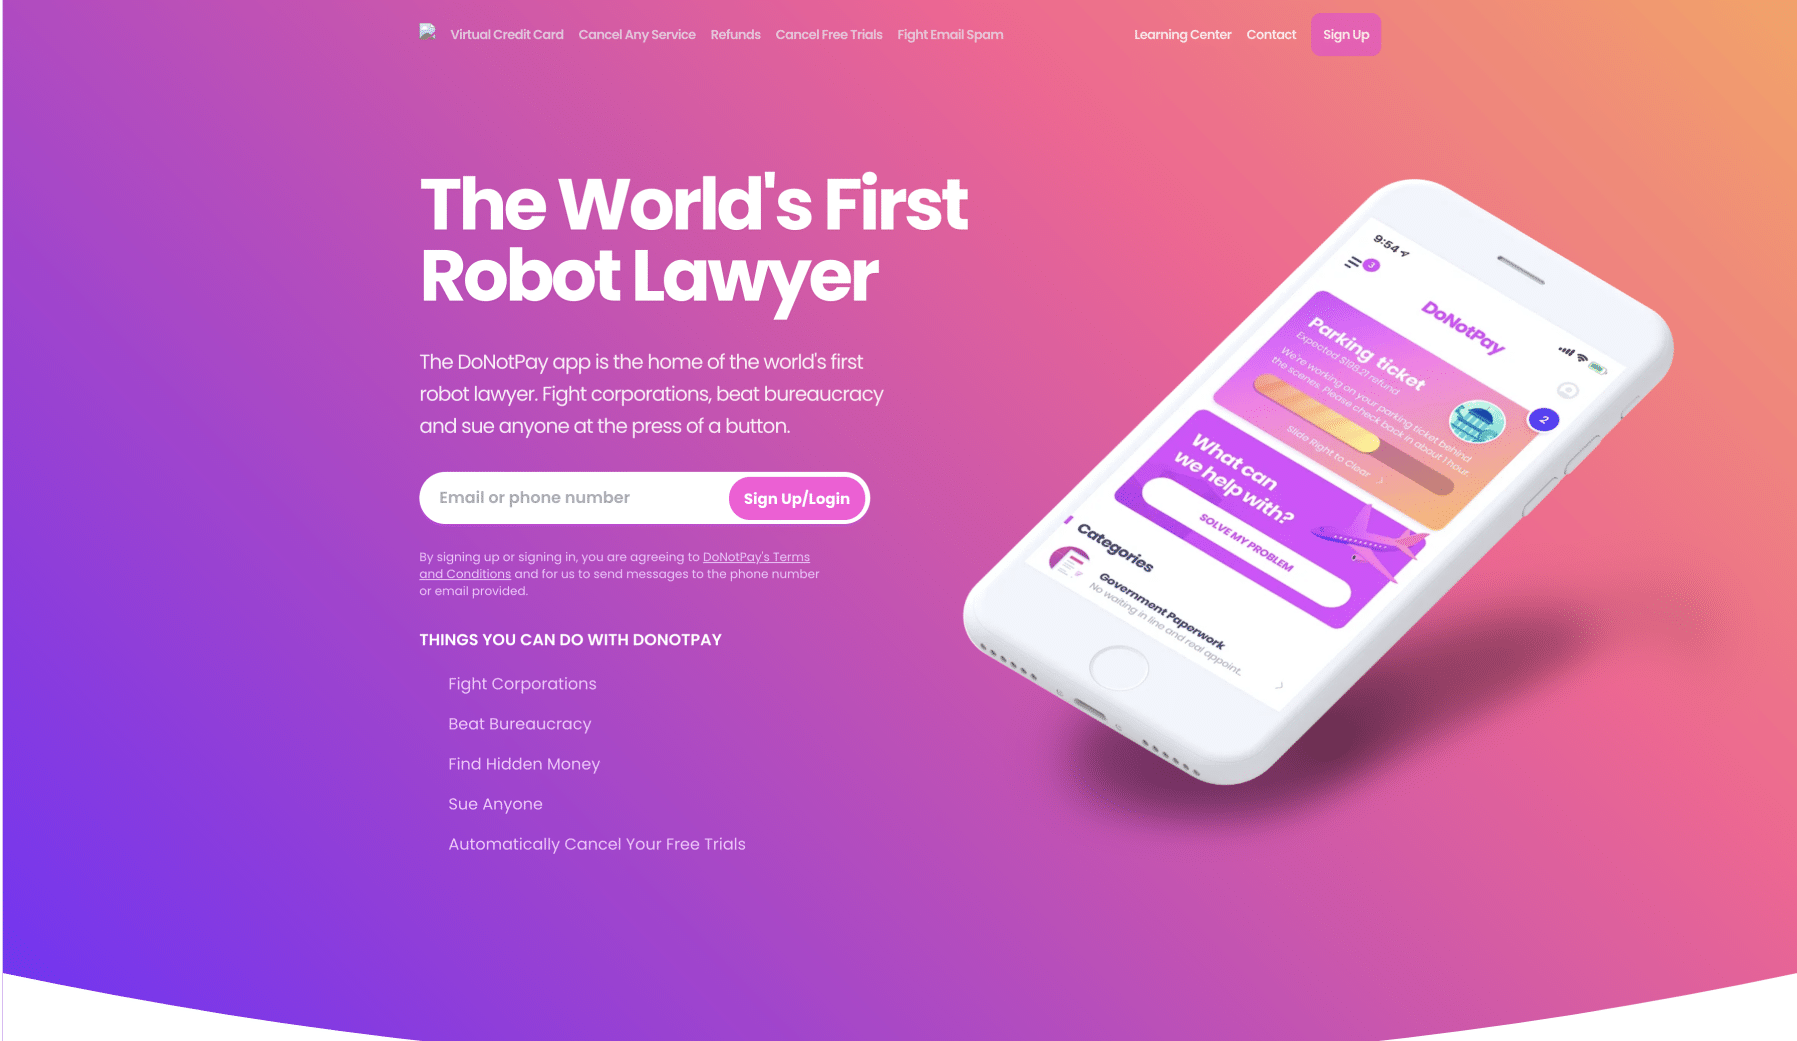
\includegraphics[width=0.8\textwidth]{donotpay_interface.png}
  \caption{Interfaz de la aplicaci\'{o}n DoNotPay.}
  \label{fig:donotpay}
\end{figure}

\textbf{2. LawBot} (Universidad de Cambridge, Reino Unido). Este sistema se orient\'{o} a brindar informaci\'{o}n legal preliminar a v\'{i}ctimas de delitos sexuales y otros delitos menores \cite{ley10426}. LawBot valid\'{o} el potencial de los sistemas conversacionales para guiar a las v\'{i}ctimas en momentos de crisis. No obstante, el proyecto no lleg\'{o} a consolidarse comercialmente y carec\'{i}a de funcionalidades cr\'{i}ticas para el contexto boliviano: integraci\'{o}n de un marco legal completo, actualizaci\'{o}n autom\'{a}tica de normativa y un grafo de relaciones entre normas jur\'{i}dicas.

\begin{figure}[H]
  \centering
  
\includegraphics[width=0.35\textwidth]{lawbot_logo.png}
  \caption{LawBot, sistema de orientaci\'{o}n legal desarrollado en Cambridge.}
  \label{fig:lawbot}
\end{figure}

\textbf{3. Microsoft Graph RAG} (Microsoft Research, 2024). \textcite{edge2024} propusieron una arquitectura que extiende el paradigma RAG mediante la construcci\'{o}n de grafos de conocimiento a partir de corpus documentales. Si bien la investigaci\'{o}n se centr\'{o} en dominios gen\'{e}ricos, demostr\'{o} que la combinaci\'{o}n de b\'{u}squeda vectorial con navegaci\'{o}n de grafo produce respuestas m\'{a}s completas y contextualizadas. LexIA adapta esta arquitectura espec\'{i}ficamente al dominio jur\'{i}dico boliviano, con un grafo que modela las relaciones reales entre leyes, decretos, art\'{i}culos, \'{a}reas del derecho y procesos legales.

A diferencia de estos antecedentes, LexIA se diferencia por: (a) su adaptaci\'{o}n espec\'{i}fica a la legislaci\'{o}n boliviana vigente obtenida autom\'{a}ticamente de la Gaceta Oficial; (b) la implementaci\'{o}n de un grafo de conocimiento legal que modela relaciones entre normas (derogaci\'{o}n, reglamentaci\'{o}n, referencia cruzada); (c) un agente con m\'{u}ltiples estados de razonamiento capaz de clasificar, clarificar y evaluar la complejidad de cada caso; y (d) un sistema de derivaci\'{o}n a abogados especializados cuando la complejidad lo requiere.

\subsection{Descripci\'{o}n del contexto}

El proyecto se desarrolla en el contexto boliviano, caracterizado por una notable asimetr\'{i}a en el acceso a la informaci\'{o}n jur\'{i}dica. A pesar de que el Estado ha promulgado normativas de Gobierno Electr\'{o}nico y Transparencia, la interfaz entre la legislaci\'{o}n y la ciudadan\'{i}a sigue siendo deficiente.

En el \'{a}mbito social, existe un desconocimiento generalizado sobre los procedimientos formales, lo que incide directamente en la baja tasa de denuncias (14,1\%) identificada en la Encuesta de Victimizaci\'{o}n \cite{tic_bolivia_2025}. En el \'{a}mbito tecnol\'{o}gico, la adopci\'{o}n de herramientas de inteligencia artificial en el sector justicia es incipiente en Bolivia. Las soluciones actuales son predominantemente repositorios est\'{a}ticos de leyes (PDFs escaneados o digitales) que no permiten una interacci\'{o}n sem\'{a}ntica ni la navegaci\'{o}n de relaciones entre normas.

La Gaceta Oficial del Estado Plurinacional de Bolivia \cite{gaceta_oficial}, fuente primaria de toda la normativa legal del pa\'{i}s, opera bajo el sistema de gesti\'{o}n de contenidos Drupal~10 con renderizado del lado del servidor, lo que permite la extracci\'{o}n automatizada de datos sin necesidad de navegadores headless. Todos los documentos publicados son PDFs con texto digital incrustado, facilitando su procesamiento computacional sin recurrir a reconocimiento \'{o}ptico de caracteres (OCR). Estas caracter\'{i}sticas t\'{e}cnicas de la fuente oficial han sido determinantes en las decisiones de dise\~{n}o del pipeline ETL de LexIA.

\section{Descripci\'{o}n del objeto de estudio}

El objeto de estudio se define como un \textbf{Sistema Inteligente de Orientaci\'{o}n Legal Conversacional basado en Graph RAG y Agentes de M\'{u}ltiples Estados}. Se trata de un artefacto de software con arquitectura web que integra cuatro capacidades fundamentales:

\begin{enumerate}
  \item \textbf{Ingesti\'{o}n automatizada de normativa:} Pipeline ETL orquestado con Prefect~3 que extrae, procesa e indexa la legislaci\'{o}n vigente desde la Gaceta Oficial de Bolivia, manteni\'{e}ndose actualizado de forma diaria sin intervenci\'{o}n manual.

  \item \textbf{Grafo de conocimiento legal:} Representaci\'{o}n expl\'{i}cita de las relaciones entre entidades jur\'{i}dicas (leyes, decretos, art\'{i}culos, \'{a}reas del derecho, procesos legales) en Neo4j, que permite la navegaci\'{o}n contextual de la normativa.

  \item \textbf{Recuperaci\'{o}n h\'{i}brida:} Motor que combina b\'{u}squeda sem\'{a}ntica vectorial (BGE-M3 + LanceDB) con expansi\'{o}n por grafo (Neo4j) y reranking mediante Cross-Encoder, produciendo un contexto normativo m\'{a}s completo y preciso que los enfoques vectoriales puros.

  \item \textbf{Agente conversacional con m\'{u}ltiples estados:} Implementado con LangGraph sobre Gemini~2.5~Flash, el agente gestiona el di\'{a}logo a trav\'{e}s de estados de clasificaci\'{o}n, clarificaci\'{o}n, recuperaci\'{o}n, evaluaci\'{o}n y respuesta, adaptando su comportamiento a la complejidad del caso.
\end{enumerate}

El sistema no pretende sustituir la asesor\'{i}a legal profesional, sino fungir como una herramienta de orientaci\'{o}n procesal primaria que reduce la incertidumbre inicial del ciudadano, le informa sobre sus derechos y, cuando la complejidad del caso lo amerita, lo deriva hacia profesionales especializados.

\section{Identificaci\'{o}n del Problema}

El acceso a la justicia en Bolivia enfrenta barreras estructurales de naturaleza informativa, econ\'{o}mica y burocr\'{a}tica. La brecha entre la incidencia real de conflictos jur\'{i}dicos y los casos efectivamente atendidos por el sistema legal evidencia una desconexi\'{o}n profunda entre la ciudadan\'{i}a y el aparato normativo.

Para analizar las causas ra\'{i}z de este fen\'{o}meno, se ha elaborado un Diagrama de Ishikawa (Causa-Efecto), ilustrado en la Figura~\ref{fig:ishikawa}.

% --- DIAGRAMA DE ISHIKAWA ---
\begin{figure}[H]
\centering
\begin{tikzpicture}[%
  spine/.style={ultra thick, ->, >=latex, draw=black!80},%
  rib/.style={thick, draw=blue!40!black},%
  category/.style={draw, rounded corners, fill=green!20, text width=2.8cm, align=center, font=\bfseries\footnotesize, drop shadow},%
  cause/.style={draw=none, fill=red!5, text width=2.5cm, align=left, font=\scriptsize, inner sep=2pt},%
  head/.style={draw, ultra thick, fill=red!10, text width=3.5cm, align=center, font=\bfseries, drop shadow, minimum height=2cm}%
]
  \draw[spine] (0,0) -- (14.5,0);
  \node[head] at (14.5,0) {BRECHA DE\\ACCESO A LA\\JUSTICIA};
  % Superior izquierda
  \draw[rib] (3,0) -- (1,3);
  \node[category] at (1,3.3) {TECNOLOG\'{I}A};
  \draw (2.3, 1.0) -- (3.5, 1.0) node[right, cause] {Sistemas obsoletos};
  \draw (1.7, 2.0) -- (2.9, 2.0) node[right, cause] {Falta de herramientas digitales};
  % Superior derecha
  \draw[rib] (9,0) -- (7,3);
  \node[category] at (7,3.3) {INFORMACI\'{O}N};
  \draw (8.3, 1.0) -- (9.5, 1.0) node[right, cause] {Datos dispersos y no centralizados};
  \draw (7.7, 2.0) -- (8.9, 2.0) node[right, cause] {Lenguaje jur\'{i}dico complejo};
  % Inferior izquierda
  \draw[rib] (3,0) -- (1,-3);
  \node[category] at (1,-3.3) {PROCESOS};
  \draw (2.3, -1.0) -- (3.5, -1.0) node[right, cause] {Burocracia excesiva en tr\'{a}mites};
  \draw (1.7, -2.0) -- (2.9, -2.0) node[right, cause] {Exigencia de presencia f\'{i}sica};
  % Inferior derecha
  \draw[rib] (9,0) -- (7,-3);
  \node[category] at (7,-3.3) {ENTORNO};
  \draw (8.3, -1.0) -- (9.5, -1.0) node[right, cause] {Saturaci\'{o}n de oficinas p\'{u}blicas};
  \draw (7.7, -2.0) -- (8.9, -2.0) node[right, cause] {Desconfianza institucional};
\end{tikzpicture}
\caption{Diagrama de Causa-Efecto (Ishikawa) sobre la brecha de acceso a la justicia.}
\label{fig:ishikawa}
\end{figure}

El an\'{a}lisis permite identificar cuatro categor\'{i}as causales principales:

\begin{itemize}
  \item \textbf{Barrera sem\'{a}ntica:} El lenguaje t\'{e}cnico de la normativa resulta inaccesible para el ciudadano promedio, quien no logra traducir su experiencia vivida a t\'{e}rminos jur\'{i}dicos aplicables.

  \item \textbf{Obsolescencia y dispersi\'{o}n:} Las leyes son modificadas frecuentemente. Los ciudadanos suelen acceder a documentos desactualizados o fragmentarios en internet, generando desinformaci\'{o}n.

  \item \textbf{Saturaci\'{o}n de canales presenciales:} La demanda excede la capacidad de atenci\'{o}n de las instituciones p\'{u}blicas, dejando a los ciudadanos sin orientaci\'{o}n preliminar.

  \item \textbf{Carencia de herramientas contextuales:} Los modelos de lenguaje comerciales (ChatGPT, Gemini) carecen de conexi\'{o}n directa y verificada con la normativa boliviana vigente, propiciando respuestas incorrectas o ``alucinaciones'' legales.
\end{itemize}

\section{Formulaci\'{o}n del Problema}

A partir del diagn\'{o}stico anterior, se formula la siguiente interrogante de investigaci\'{o}n:

\textbf{?`C\'{o}mo dise\~{n}ar e implementar un sistema de orientaci\'{o}n legal conversacional que, mediante t\'{e}cnicas de inteligencia artificial y un grafo de conocimiento jur\'{i}dico, proporcione informaci\'{o}n normativa fundada, actualizada y contextualizada a la legislaci\'{o}n boliviana vigente, haciendo ese conocimiento accesible para cualquier ciudadano con independencia de su formaci\'{o}n jur\'{i}dica?}

\section{Objetivos}

\subsection{Objetivo General}

Desarrollar LexIA, un sistema de orientaci\'{o}n legal conversacional para Bolivia que integre \textit{Graph RAG} y agentes inteligentes con m\'{u}ltiples estados de razonamiento, para proporcionar informaci\'{o}n jur\'{i}dica contextualizada, fundamentada en la legislaci\'{o}n vigente y accesible a usuarios sin formaci\'{o}n jur\'{i}dica especializada.

\subsection{Objetivos Espec\'{i}ficos}

\begin{itemize}
  \item \textbf{Desarrollar} un pipeline ETL automatizado con Prefect~3 que extraiga, procese e indexe la normativa publicada en la Gaceta Oficial de Bolivia, actualiz\'{a}ndose peri\'{o}dicamente ante nuevas publicaciones.

  \item \textbf{Construir} un grafo de conocimiento legal en Neo4j que represente las relaciones jur\'{i}dicas entre leyes, decretos, art\'{i}culos, \'{a}reas del derecho y procesos legales de Bolivia.

  \item \textbf{Implementar} un motor de recuperaci\'{o}n h\'{i}brida que combine b\'{u}squeda sem\'{a}ntica vectorial (LanceDB + BGE-M3) con expansi\'{o}n por grafo (Neo4j) y reranking mediante Cross-Encoder.

  \item \textbf{Desarrollar} un agente conversacional con LangGraph que gestione el di\'{a}logo a trav\'{e}s de estados de razonamiento diferenciados, adapt\'{a}ndose a la complejidad jur\'{i}dica de cada consulta.

  \item \textbf{Construir} una interfaz web accesible mediante Next.js~14 que permita interacci\'{o}n en lenguaje natural, incluyendo modalidad de acceso para invitados sin registro previo.

  \item \textbf{Evaluar} el desempe\~{n}o del sistema con el framework RAGAS, comparando \textit{Graph RAG} frente a RAG est\'{a}ndar en m\'{e}tricas de fidelidad, relevancia y completitud.
\end{itemize}

\section{Justificaciones}

\subsection{Justificaci\'{o}n t\'{e}cnica}

El proyecto aporta valor acad\'{e}mico y t\'{e}cnico al implementar una arquitectura de \textbf{Graph RAG} ---una extensi\'{o}n del paradigma RAG convencional que incorpora grafos de conocimiento en el proceso de recuperaci\'{o}n---. A diferencia de los sistemas est\'{a}ticos, la incorporaci\'{o}n de un pipeline ETL automatizado con Prefect introduce un componente de ingenier\'{i}a de datos avanzado que permite la actualizaci\'{o}n continua sin reentrenamiento de modelos. El uso de un grafo de conocimiento legal en Neo4j, combinado con b\'{u}squeda vectorial en LanceDB y embeddings locales BGE-M3, representa una aplicaci\'{o}n moderna de la recuperaci\'{o}n de informaci\'{o}n en el \'{a}mbito legal boliviano que no tiene precedentes en el contexto local.

\subsection{Justificaci\'{o}n social}

La herramienta se alinea con el principio constitucional de democratizaci\'{o}n del acceso a la justicia. Al poner una herramienta de orientaci\'{o}n legal gratuita y actualizada al alcance de cualquier dispositivo con conexi\'{o}n a internet, se reduce la brecha de indefensi\'{o}n que afecta a los sectores que no pueden costear asesor\'{i}a legal privada para consultas iniciales. Facilitar el acceso a la informaci\'{o}n jur\'{i}dica es un paso fundamental para visibilizar la realidad de los conflictos legales y reducir la impunidad derivada de la desinformaci\'{o}n.

\subsection{Justificaci\'{o}n econ\'{o}mica}

La arquitectura del sistema prioriza el uso de tecnolog\'{i}as de c\'{o}digo abierto: Neo4j Community Edition, LanceDB, BGE-M3 (ejecuci\'{o}n local), Prefect~3, FastAPI, Next.js~14 y Docker Compose. El \'{u}nico componente de pago es la API de Gemini~2.5~Flash, cuyo costo por token es competitivo en comparaci\'{o}n con alternativas como GPT-4o o Claude. La estimaci\'{o}n de costos operativos mensuales no supera los \$35 USD, haciendo viable su sostenimiento incluso como proyecto acad\'{e}mico sin financiamiento externo.

\section{L\'{i}mites y Alcances}

\subsection{L\'{i}mites}

\begin{itemize}
  \item \textbf{Fuentes de datos:} El pipeline de extracci\'{o}n se limita a la Gaceta Oficial de Bolivia, procesando \'{u}nicamente PDFs con texto digital (no im\'{a}genes escaneadas).
  \item \textbf{Cobertura temporal:} Normativa publicada desde el a\~{n}o 2010 hasta la fecha de implementaci\'{o}n.
  \item \textbf{Responsabilidad:} El sistema incluye descargos expl\'{i}citos, aclarando que la informaci\'{o}n es orientativa y no constituye asesor\'{i}a legal vinculante.
  \item \textbf{Jurisprudencia:} Las sentencias de los tribunales bolivianos no est\'{a}n incluidas en la versi\'{o}n actual.
  \item \textbf{Datos personales:} El sistema no almacena informaci\'{o}n personal identificable (PII) de los usuarios en las sesiones de invitado.
\end{itemize}

\subsection{Alcances}

\begin{itemize}
  \item Implementaci\'{o}n de un pipeline ETL completo (Extracci\'{o}n, Transformaci\'{o}n, Carga e Indexaci\'{o}n) con Prefect~3, httpx y BeautifulSoup4.
  \item Construcci\'{o}n de un grafo de conocimiento legal con 9~\'{a}reas del derecho, relaciones de derogaci\'{o}n, reglamentaci\'{o}n y referencia cruzada en Neo4j.
  \item Desarrollo de una interfaz conversacional responsiva con Next.js~14, TailwindCSS y ShadcnUI.
  \item API REST con FastAPI, autenticaci\'{o}n JWT y modalidad de acceso para invitados (l\'{i}mite de 3~consultas).
  \item Sistema de derivaci\'{o}n a abogados especializados integrado en el flujo del agente.
  \item Evaluaci\'{o}n comparativa de calidad de respuestas con el framework RAGAS.
\end{itemize}

\section{Metodolog\'{i}a de la investigaci\'{o}n}

\subsection{Tipo de estudio}

El presente trabajo adopta un enfoque de \textbf{investigaci\'{o}n aplicada con desarrollo de prototipo funcional}. El tipo de estudio es descriptivo-exploratorio: descriptivo en cuanto caracteriza la problem\'{a}tica del acceso a la informaci\'{o}n legal en Bolivia y las limitaciones de las soluciones existentes; exploratorio en cuanto introduce una arquitectura t\'{e}cnica (\textit{Graph RAG} sobre legislaci\'{o}n boliviana) que no tiene precedentes documentados en el contexto local.

\subsection{M\'{e}todos}

Se emplean los siguientes m\'{e}todos de investigaci\'{o}n:

\begin{itemize}
  \item \textbf{M\'{e}todo anal\'{i}tico-sint\'{e}tico:} Descomposici\'{o}n del problema del acceso a la justicia en sus componentes informativo, tecnol\'{o}gico, procedimental e institucional, para luego sintetizar una soluci\'{o}n integral.
  \item \textbf{M\'{e}todo experimental:} Evaluaci\'{o}n comparativa entre dos configuraciones del sistema (RAG est\'{a}ndar vs.\ Graph RAG) mediante m\'{e}tricas objetivas del framework RAGAS.
  \item \textbf{M\'{e}todo de desarrollo \'{a}gil:} Implementaci\'{o}n iterativa en seis fases con entregables verificables al cierre de cada una.
\end{itemize}

\subsection{T\'{e}cnicas}

Las t\'{e}cnicas de recolecci\'{o}n y procesamiento de informaci\'{o}n incluyen: revisi\'{o}n documental de la normativa boliviana publicada en la Gaceta Oficial; an\'{a}lisis estad\'{i}stico de las encuestas de victimizaci\'{o}n y acceso a la justicia; extracci\'{o}n automatizada de datos mediante web scraping; y evaluaci\'{o}n cuantitativa de la calidad de las respuestas generadas por el sistema.

\section{An\'{a}lisis preliminar}

El an\'{a}lisis de la situaci\'{o}n actual revela que la brecha de acceso a la justicia en Bolivia opera en tres dimensiones convergentes. Primero, una \textbf{brecha sem\'{a}ntica}: el ciudadano describe su situaci\'{o}n en lenguaje coloquial mientras la normativa est\'{a} redactada en terminolog\'{i}a jur\'{i}dica t\'{e}cnica; los sistemas convencionales de b\'{u}squeda por palabras clave no pueden resolver esta discrepancia de vocabulario \cite{manning2008}. Segundo, una \textbf{brecha temporal}: las leyes son modificadas, derogadas y reglamentadas continuamente, pero los repositorios est\'{a}ticos de documentos legales no reflejan estas actualizaciones. Tercero, una \textbf{brecha relacional}: una norma no existe en aislamiento sino en un entramado de relaciones con otras normas ---cita, modifica, deroga, reglamenta--- que los sistemas de recuperaci\'{o}n vectorial puros no modelan.

Las soluciones disponibles actualmente ---modelos de lenguaje comerciales sin conexi\'{o}n a la normativa boliviana, repositorios est\'{a}ticos de PDFs, consultas presenciales en oficinas saturadas--- son insuficientes para abordar estas tres dimensiones simult\'{a}neamente.

\section{Propuesta de soluci\'{o}n}

La propuesta consiste en el desarrollo de LexIA, un sistema que resuelve las tres brechas identificadas mediante la integraci\'{o}n de:

\begin{enumerate}
  \item Un \textbf{pipeline ETL automatizado} que mantiene la base de conocimiento sincronizada con la Gaceta Oficial (resuelve la brecha temporal).
  \item Un \textbf{motor de embeddings sem\'{a}nticos} (BGE-M3) que permite la b\'{u}squeda por significado, no por coincidencia de palabras (resuelve la brecha sem\'{a}ntica).
  \item Un \textbf{grafo de conocimiento legal} en Neo4j que modela expl\'{i}citamente las relaciones entre normas (resuelve la brecha relacional).
  \item Un \textbf{agente conversacional} con LangGraph que orquesta el di\'{a}logo y adapta su comportamiento a la complejidad del caso.
\end{enumerate}

La Figura~\ref{fig:conceptual_solution} modela la transformaci\'{o}n conceptual que el sistema introduce.

\begin{figure}[H]
\centering
\begin{tikzpicture}[%
  node distance=2.5cm,%
  problem/.style={rectangle, draw=red!60!black, top color=white, bottom color=red!10, text width=4cm, text centered, rounded corners, minimum height=2.5cm, font=\small},%
  solution/.style={rectangle, draw=green!60!black, top color=white, bottom color=green!10, text width=4cm, text centered, rounded corners, minimum height=2.5cm, font=\small},%
  system/.style={circle, draw=blue!60!black, top color=white, bottom color=blue!10, text width=2.8cm, text centered, minimum height=2.8cm, circular drop shadow, font=\bfseries},%
  arrow/.style={->, >=latex, ultra thick, draw=gray!80, text=black}%
]
  \node[problem] (actual) {\textbf{ESTADO ACTUAL}\\(Asimetr\'{i}a)\\ \rule{3.5cm}{0.4pt} \\ \footnotesize Normas dispersas\\Lenguaje t\'{e}cnico\\Sin relaciones};
  \node[system, right=2.2cm of actual] (chatbot) {LexIA\\Graph RAG\\+ Agente};
  \node[solution, right=2.2cm of chatbot] (futuro) {\textbf{ESTADO FUTURO}\\(Acceso Efectivo)\\ \rule{3.5cm}{0.4pt} \\ \footnotesize Orientaci\'{o}n precisa\\Citas verificadas\\Derivaci\'{o}n profesional};
  \draw[arrow] (actual) -- node[above, font=\scriptsize, align=center, yshift=0.1cm] {Consulta en\\Lenguaje Natural} (chatbot);
  \draw[arrow] (chatbot) -- node[above, font=\scriptsize, align=center, yshift=0.1cm] {Orientaci\'{o}n Legal\\Fundamentada} (futuro);
\end{tikzpicture}
\caption{Modelo conceptual de la transformaci\'{o}n del acceso a la informaci\'{o}n legal.}
\label{fig:conceptual_solution}
\end{figure}

\section{Modelos y herramientas a utilizar}

\begin{table}[H]
  \centering
  \renewcommand{\arraystretch}{1.3}
  \caption{Modelos de ingenier\'{i}a aplicados al proyecto.}
  \label{tab:modelos_ing}
  \begin{tabular}{|p{0.3\textwidth}|p{0.6\textwidth}|}
  \hline
  \textbf{Modelo} & \textbf{Descripci\'{o}n y Aplicaci\'{o}n} \\ \hline
  Modelo C4 & Documentaci\'{o}n de la arquitectura en niveles: Contexto, Contenedores, Componentes y C\'{o}digo. \\ \hline
  UML 2.5 (Secuencia, Clases, Actividades) & Modelado del flujo de datos entre el pipeline ETL, el agente LangGraph, la API FastAPI y el frontend Next.js. \\ \hline
  Metodolog\'{i}a \'{A}gil Iterativa & Desarrollo en seis fases incrementales con entregables verificables por fase. \\ \hline
  \end{tabular}
\end{table}

\begin{table}[H]
  \centering
  \renewcommand{\arraystretch}{1.3}
  \caption{Stack tecnol\'{o}gico del sistema LexIA.}
  \label{tab:herramientas_tec}
  \begin{tabular}{|p{0.22\textwidth}|p{0.25\textwidth}|p{0.43\textwidth}|}
  \hline
  \textbf{Categor\'{i}a} & \textbf{Tecnolog\'{i}a} & \textbf{Justificaci\'{o}n} \\ \hline
  Scraper Web & httpx 0.27 + BeautifulSoup4 & Gaceta Oficial usa Drupal 10 SSR; no requiere navegador headless. \\ \hline
  Extracci\'{o}n PDF & PyMuPDF + pdfplumber & PDFs digitales; cascada de extractores sin necesidad de OCR. \\ \hline
  Embeddings & BGE-M3 (1024 dims) & Multiling\"{u}e, ejecuci\'{o}n local, sin API externa, gratuito. \\ \hline
  Base Vectorial & LanceDB 0.17 & Sin servidor dedicado, wheels precompilados para Windows. \\ \hline
  Grafo de Conocimiento & Neo4j 5.18 Community & Est\'{a}ndar de la industria; Cypher declarativo; plugin APOC. \\ \hline
  Orquestaci\'{o}n ETL & Prefect 3.1 & Scheduling, reintentos autom\'{a}ticos, cach\'{e} y observabilidad. \\ \hline
  Backend / API & FastAPI 0.115 & OpenAPI autom\'{a}tico, validaci\'{o}n Pydantic, alto rendimiento ASGI. \\ \hline
  Agente IA & LangGraph 0.2 & Grafo de estados expl\'{i}cito, depurable, soporte streaming. \\ \hline
  Modelo de Lenguaje & Gemini 2.5 Flash & 1M tokens contexto, bajo costo, alta capacidad multiling\"{u}e. \\ \hline
  BD Relacional & PostgreSQL 16 + SQLAlchemy 2 & Persistencia de usuarios, conversaciones y mensajes. \\ \hline
  Autenticaci\'{o}n & python-jose + passlib & JWT est\'{a}ndar, bcrypt para contrase\~{n}as. \\ \hline
  Cach\'{e} & Redis 7 & Cach\'{e} de embeddings frecuentes y sesiones. \\ \hline
  Frontend & Next.js 14 + TailwindCSS + ShadcnUI & SSR, React Server Components, dise\~{n}o responsivo. \\ \hline
  Infraestructura & Docker Compose & PostgreSQL, Redis y Neo4j contenedorizados. \\ \hline
  \end{tabular}
\end{table}

\section{Cronograma}

La planificaci\'{o}n temporal se estructura en seis fases alineadas con el calendario del Taller de Grado~II:

\begin{enumerate}
  \item \textbf{Fase 1: Ingenier\'{i}a de Datos (Semanas 1--4):} Pipeline ETL, scraper, extracci\'{o}n de texto, embeddings, indexaci\'{o}n en LanceDB y Neo4j.
  \item \textbf{Fase 2: Backend y Agente (Semanas 5--8):} API REST con FastAPI, agente LangGraph, autenticaci\'{o}n JWT, servicios de chat.
  \item \textbf{Fase 3: Frontend (Semanas 9--11):} Interfaz conversacional con Next.js~14, integraci\'{o}n con API, historial de conversaciones.
  \item \textbf{Fase 4: Integraci\'{o}n y Pruebas (Semanas 12--14):} Pruebas de integraci\'{o}n, evaluaci\'{o}n RAGAS, ajuste de prompts.
  \item \textbf{Fase 5: Despliegue (Semanas 15--16):} Docker Compose completo, documentaci\'{o}n t\'{e}cnica.
  \item \textbf{Fase 6: Documentaci\'{o}n y Defensa (Semanas 17--18):} Redacci\'{o}n final del documento, preparaci\'{o}n de la sustentaci\'{o}n.
\end{enumerate}

\begin{figure}[H]
  \centering
  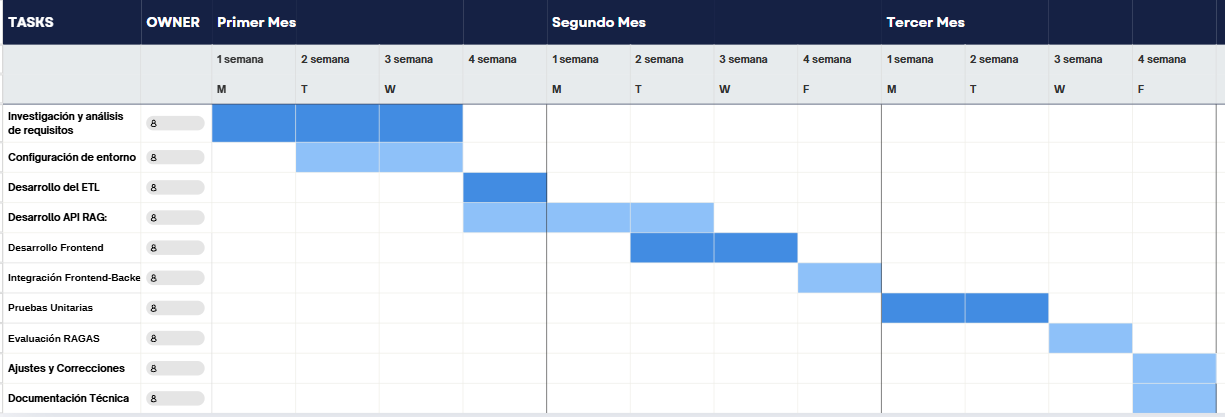
\includegraphics[width=1.0\textwidth]{cronograma_gantt.png}
  \caption{Diagrama de Gantt: Cronograma de implementaci\'{o}n para Taller de Grado~II.}
  \label{fig:cronograma}
\end{figure}


% ====================== CAPITULO 2 ======================
\chapter{Marco Te\'{o}rico}

\section{Metodolog\'{i}a de an\'{a}lisis y dise\~{n}o}

El an\'{a}lisis del sistema se fundamenta en el modelo C4 de Simon Brown para la documentaci\'{o}n arquitect\'{o}nica y en UML~2.5 para el modelado de comportamiento y estructura. El modelo C4 organiza la arquitectura en cuatro niveles de abstracci\'{o}n ---Contexto, Contenedores, Componentes y C\'{o}digo--- facilitando la comunicaci\'{o}n de las decisiones de dise\~{n}o a audiencias con distintos niveles de profundidad t\'{e}cnica \cite{booch2005}.

\section{Metodolog\'{i}a de desarrollo}

El proyecto adopta una \textbf{metodolog\'{i}a \'{a}gil adaptada a sistemas de inteligencia artificial}. A diferencia de las metodolog\'{i}as cascada tradicionales, el desarrollo de sistemas basados en LLM y RAG requiere ciclos iterativos de experimentaci\'{o}n: la calidad de las respuestas depende de la interacci\'{o}n entre los prompts, el contexto recuperado y los par\'{a}metros del modelo, variables que solo pueden optimizarse emp\'{i}ricamente. El desarrollo se organiza en seis fases iterativas con entregables tangibles e hitos de control al cierre de cada una.

\section{Fundamentos de Inteligencia Artificial}

\subsection{Modelos de Lenguaje de Gran Escala (LLM)}

Los Modelos de Lenguaje de Gran Escala son sistemas de aprendizaje profundo entrenados sobre corpus textuales masivos mediante objetivos autosupervisados de predicci\'{o}n de secuencias. La arquitectura \textit{Transformer}, introducida por \textcite{vaswani2017}, basada en mecanismos de atenci\'{o}n multi-cabeza que modelan dependencias a larga distancia en el texto, se ha consolidado como el paradigma dominante para esta clase de modelos. Operan como motores probabil\'{i}sticos que, dado un contexto de entrada, predicen la continuaci\'{o}n m\'{a}s probable ponderando la relevancia de cada token de la secuencia mediante el mecanismo de auto-atenci\'{o}n \cite{russell2010}.

En el contexto del presente proyecto, el LLM empleado es \textbf{Gemini~2.5~Flash}, seleccionado por tres caracter\'{i}sticas cr\'{i}ticas: su ventana de contexto de un mill\'{o}n de tokens (suficiente para incorporar vol\'{u}menes significativos de normativa), su alta competencia con el espa\~{n}ol latinoamericano, y su bajo costo por token frente a alternativas de mayor tama\~{n}o. La funci\'{o}n del LLM en LexIA es estrictamente generativa: sintetiza y reformula la informaci\'{o}n jur\'{i}dica inyectada mediante el contexto recuperado, sin actuar como almac\'{e}n de conocimiento f\'{a}ctico.

\subsection{Alucinaci\'{o}n Artificial}

El fen\'{o}meno de alucinaci\'{o}n en modelos generativos ---la producci\'{o}n de afirmaciones gramaticalmente coherentes pero factualmente incorrectas--- constituye un riesgo cr\'{i}tico en el dominio legal \cite{maynez2020}. La arquitectura RAG act\'{u}a como capa de restricci\'{o}n (\textit{grounding}), forzando al modelo a derivar su respuesta exclusivamente de los fragmentos normativos recuperados de la base de datos, minimizando la probabilidad de invenci\'{o}n jur\'{i}dica. La evaluaci\'{o}n de fidelidad mediante RAGAS permite cuantificar objetivamente la incidencia residual de alucinaciones.

\subsection{Generaci\'{o}n Aumentada por Recuperaci\'{o}n (RAG)}

La Generaci\'{o}n Aumentada por Recuperaci\'{o}n, propuesta por \textcite{lewis2020}, optimiza la salida de un LLM al referenciar una base de conocimientos autorizada antes de generar una respuesta. A diferencia del reentrenamiento (\textit{Fine-Tuning}), que almacena el conocimiento en los par\'{a}metros de la red neuronal, el enfoque RAG recupera informaci\'{o}n en tiempo real desde fuentes verificables.

\begin{table}[H]
  \centering
  \renewcommand{\arraystretch}{1.3}
  \caption{Comparaci\'{o}n t\'{e}cnica: RAG vs.\ Fine-Tuning para dominios legales.}
  \label{tab:rag_vs_finetuning}
  \begin{tabular}{|p{0.25\textwidth}|p{0.35\textwidth}|p{0.3\textwidth}|}
  \hline
  \textbf{Criterio} & \textbf{RAG (Seleccionada)} & \textbf{Fine-Tuning (Descartada)} \\ \hline
  Actualizaci\'{o}n & Din\'{a}mica. Basta con actualizar la base vectorial y el grafo. & Est\'{a}tica. Requiere reentrenar el modelo. \\ \hline
  Alucinaciones & Bajas. El modelo se restringe al contexto recuperado. & Medias/Altas. El modelo puede inventar hechos. \\ \hline
  Trazabilidad & Alta. Se puede citar la fuente exacta. & Baja. Es una ``caja negra''. \\ \hline
  Costo & Bajo. Solo inferencia + almacenamiento. & Alto. GPU intensivo para entrenamiento. \\ \hline
  \end{tabular}
\end{table}

\subsection{Graph RAG: Recuperaci\'{o}n Aumentada sobre Grafo}

\textit{Graph RAG} extiende el paradigma RAG incorporando la navegaci\'{o}n expl\'{i}cita de grafos de conocimiento en el proceso de recuperaci\'{o}n \cite{edge2024}. La motivaci\'{o}n es que la similitud sem\'{a}ntica vectorial no captura las relaciones estructurales entre entidades. En el dominio legal, esto es cr\'{i}tico: un art\'{i}culo del C\'{o}digo Penal puede estar modificado por una ley posterior, remitirse a un art\'{i}culo del C\'{o}digo de Procedimiento Penal, y ser aplicable en un \'{a}rea del derecho que comparte normativa con legislaci\'{o}n tributaria. Un sistema que no modele estas relaciones produce respuestas necesariamente incompletas.

El retriever h\'{i}brido de LexIA ejecuta tres operaciones secuenciales: b\'{u}squeda vectorial (BGE-M3 + LanceDB), expansi\'{o}n por grafo (Neo4j) y reranking (Cross-Encoder), combinando la precisi\'{o}n sem\'{a}ntica con la completitud relacional.

\subsection{Embeddings Sem\'{a}nticos y Bases de Datos Vectoriales}

Los \textit{embeddings} son representaciones num\'{e}ricas de unidades textuales en espacios vectoriales de alta dimensi\'{o}n, dise\~{n}adas para que textos sem\'{a}nticamente pr\'{o}ximos queden geom\'{e}tricamente cercanos \cite{reimers2019}. La medida de Similitud del Coseno permite calcular la distancia angular entre el vector de la consulta del usuario y los vectores de los fragmentos normativos, habilitando la recuperaci\'{o}n basada en significado y no solo en coincidencia sint\'{a}ctica.

Para LexIA se emplea \textbf{BGE-M3} \cite{chen2024bge}, un modelo que genera vectores de 1024 dimensiones con soporte para m\'{a}s de 100~idiomas. Opera completamente en local, preservando la confidencialidad de las consultas. Los vectores se indexan en \textbf{LanceDB}, base de datos vectorial que opera sin servidor dedicado en formato Apache Lance.

\subsection{Bases de Datos de Grafos: Neo4j}

Las bases de datos de grafos representan la informaci\'{o}n como nodos y aristas, siendo superiores a los modelos relacionales cuando las conexiones entre entidades constituyen el dato primario \cite{robinson2015}. Neo4j implementa el modelo de grafo de propiedades etiquetadas con lenguaje de consulta Cypher \cite{neo4j2024}. En LexIA, el grafo modela: normas legales, art\'{i}culos, \'{a}reas del derecho, procesos legales y abogados, con relaciones de derogaci\'{o}n, reglamentaci\'{o}n, referencia cruzada y especializaci\'{o}n.

\subsection{LangGraph y Agentes de M\'{u}ltiples Estados}

LangGraph es un framework de c\'{o}digo abierto que permite modelar el razonamiento de un agente como un grafo dirigido de estados \cite{langgraph2024}. Cada nodo es una funci\'{o}n de transformaci\'{o}n del estado de la conversaci\'{o}n; cada arista es una condici\'{o}n de transici\'{o}n. Esta representaci\'{o}n expl\'{i}cita hace que el comportamiento del agente sea predecible, depurable e inspeccionable, a diferencia de los enfoques basados exclusivamente en prompts.

\subsection{Proceso ETL y Web Scraping}

Para garantizar la vigencia de la normativa, se define un proceso ETL automatizado. El sistema consulta la Gaceta Oficial de Bolivia \cite{gaceta_oficial} mediante \texttt{httpx} (cliente HTTP as\'{i}ncrono) y \texttt{BeautifulSoup4} (parser HTML). La orquestaci\'{o}n del pipeline se realiza con Prefect~3, que proporciona scheduling, reintentos autom\'{a}ticos, cach\'{e} de resultados intermedios y observabilidad integrada.

\begin{figure}[H]
  \centering
  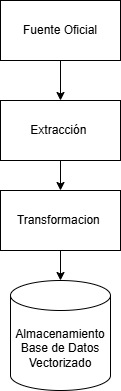
\includegraphics[width=0.1\textwidth]{diagrama_etl.png}
  \caption{Diagrama del proceso ETL para la normativa legal.}
  \label{fig:diagrama_etl}
\end{figure}

\section{Fundamentos Jur\'{i}dicos}

\subsection{LegalTech y Acceso a la Justicia}

Seg\'{u}n la CEPAL \cite{cepal2021}, la transformaci\'{o}n digital en los sistemas judiciales no es meramente t\'{e}cnica, sino que constituye un mecanismo clave para reducir las brechas de desigualdad social. El modelo de ``Justicia Digital Asistida'' propuesto por \textcite{susskind2019} establece que los sistemas tecnol\'{o}gicos no generan derecho sustantivo ni sustituyen el juicio humano; su funci\'{o}n es estrictamente instrumental: reducen la complejidad de la navegaci\'{o}n legal para el usuario final.

\subsection{Marco Normativo Boliviano}

LexIA abarca la normativa publicada en la Gaceta Oficial que cubre ocho \'{a}reas del derecho. La Tabla~\ref{tab:marco_normativo} detalla los principales cuerpos legales que conforman la base de conocimiento.

\begin{table}[H]
  \centering
  \renewcommand{\arraystretch}{1.4}
  \caption{Cuerpos legales principales que conforman la base de conocimiento.}
  \label{tab:marco_normativo}
  \begin{tabular}{|p{0.3\textwidth}|p{0.2\textwidth}|p{0.4\textwidth}|}
  \hline
  \textbf{Cuerpo Legal} & \textbf{Referencia} & \textbf{Funci\'{o}n en el Sistema} \\ \hline
  Constituci\'{o}n Pol\'{i}tica del Estado & Arts.~115, 119 & Derechos fundamentales y garant\'{i}as del debido proceso. \\ \hline
  C\'{o}digo Penal & Ley N\textdegree{} 10426 & Tipificaci\'{o}n de delitos y sanciones. \\ \hline
  C\'{o}digo de Procedimiento Penal & Ley N\textdegree{} 1970 & Flujos, plazos y requisitos procesales. \\ \hline
  Ley General del Trabajo & D.S.~21060 y modificaciones & Derechos y obligaciones laborales. \\ \hline
  C\'{o}digo Civil & D.L.~12760 & Contratos, propiedad, obligaciones civiles. \\ \hline
  C\'{o}digo Tributario & Ley N\textdegree{} 2492 & Obligaciones tributarias y procedimientos fiscales. \\ \hline
  \end{tabular}
\end{table}

\section{Tecnolog\'{i}as de Soporte}

\subsection{FastAPI}

Framework Python para APIs REST de alto rendimiento, basado en el est\'{a}ndar OpenAPI y el sistema de anotaciones de tipos. Su inyecci\'{o}n de dependencias, validaci\'{o}n autom\'{a}tica con Pydantic y soporte nativo para operaciones as\'{i}ncronas lo hacen adecuado para el backend de LexIA \cite{fielding2000}.

\subsection{Next.js 14}

Framework React con renderizado del lado del servidor (SSR) y React Server Components. Combinado con TailwindCSS y ShadcnUI, proporciona una interfaz profesional, responsiva y accesible.

\subsection{Docker y Contenedorizaci\'{o}n}

La contenedorizaci\'{o}n permite ejecutar aplicaciones en espacios aislados que comparten el kernel del sistema operativo anfitri\'{o}n \cite{merkel2014}. Docker Compose orquesta los servicios de PostgreSQL~16, Redis~7 y Neo4j~5.18, garantizando la paridad entre entornos de desarrollo y producci\'{o}n.

\subsection{Infraestructura en la Nube}

\begin{figure}[H]
  \centering
  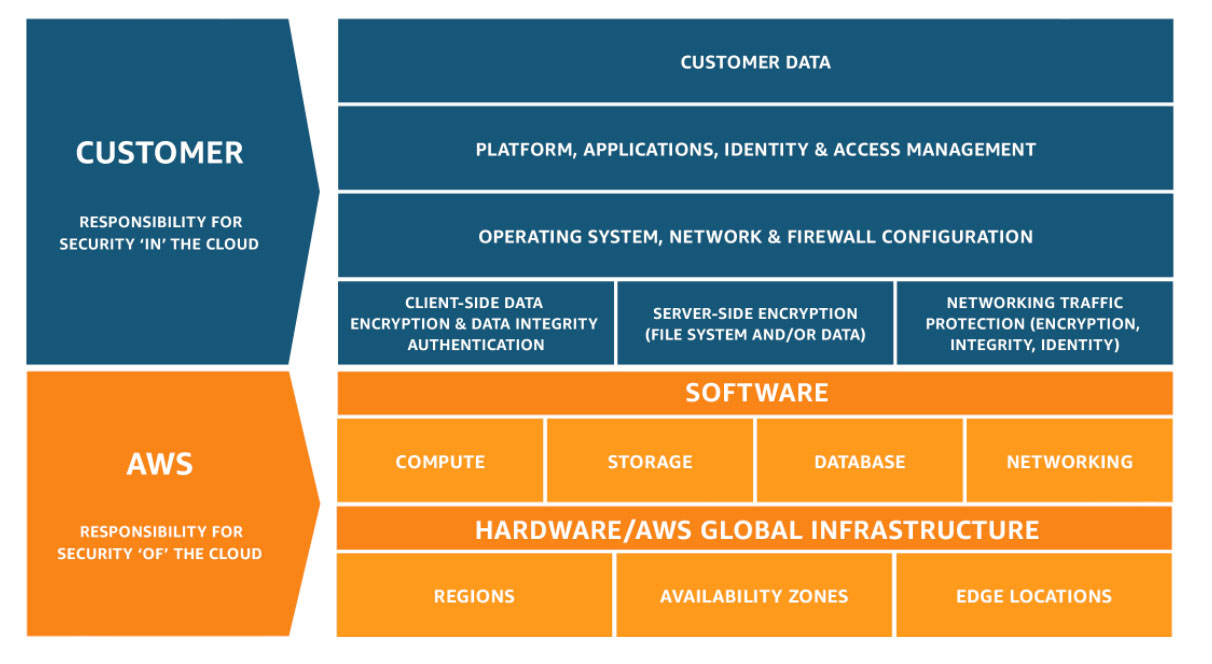
\includegraphics[width=0.7\textwidth]{cloud_model.png}
  \caption{Modelo de Responsabilidad Compartida en la Nube.}
  \label{fig:cloud_model}
\end{figure}


% ====================== CAPITULO 3 ======================
\chapter{Marco Pr\'{a}ctico}

\section{An\'{a}lisis preliminar}

El desarrollo de LexIA aborda un desaf\'{i}o de ingenier\'{i}a que opera en tres dimensiones simult\'{a}neas: la \textbf{brecha sem\'{a}ntica} entre el lenguaje natural del ciudadano y la terminolog\'{i}a jur\'{i}dica formal, la \textbf{brecha temporal} entre la normativa vigente y las fuentes estancadas disponibles en l\'{i}nea, y la \textbf{brecha relacional} entre normas interconectadas que los sistemas de recuperaci\'{o}n vectorial puros no modelan.

La arquitectura del flujo de datos se ha dise\~{n}ado bajo un paradigma de \textbf{procesamiento en etapas secuenciales} (pipeline). La Figura~\ref{fig:pipeline_rag} ilustra este flujo.

\begin{figure}[H]
\centering
\begin{tikzpicture}[%
  node distance=1.2cm and 0.6cm, auto,%
  stage/.style={rectangle, draw=blue!40!black, top color=white, bottom color=blue!5, text width=4.5em, text centered, rounded corners, minimum height=3.5em, font=\footnotesize\bfseries, drop shadow},%
  desc/.style={text width=5.5em, text centered, font=\scriptsize, yshift=-0.5cm},%
  myarrow/.style={->, >=latex', shorten >=1pt, thick, draw=blue!40!black}%
]
  \node[stage] (p1) {1. Entrada};
  \node[stage, right=of p1] (p2) {2. Clasificaci\'{o}n};
  \node[stage, right=of p2] (p3) {3. Recuperaci\'{o}n H\'{i}brida};
  \node[stage, right=of p3] (p4) {4. Evaluaci\'{o}n};
  \node[stage, right=of p4, bottom color=green!10] (p5) {5. Respuesta};
  \node[desc, below=of p1] {Consulta en lenguaje natural};
  \node[desc, below=of p2] {\'{A}rea legal + clarificaci\'{o}n};
  \node[desc, below=of p3] {LanceDB + Neo4j + CrossEncoder};
  \node[desc, below=of p4] {Complejidad del caso};
  \node[desc, below=of p5] {Orientaci\'{o}n o derivaci\'{o}n};
  \draw[myarrow] (p1) -- (p2);
  \draw[myarrow] (p2) -- (p3);
  \draw[myarrow] (p3) -- (p4);
  \draw[myarrow] (p4) -- (p5);
\end{tikzpicture}
\caption{Diagrama del pipeline de procesamiento de consultas legales (Graph RAG).}
\label{fig:pipeline_rag}
\end{figure}

\section{Determinaci\'{o}n de requerimientos}

\subsection{Requerimientos funcionales}

\begin{table}[H]
  \centering
  \renewcommand{\arraystretch}{1.3}
  \caption{Especificaci\'{o}n de Requerimientos Funcionales.}
  \label{tab:req_funcionales}
  \begin{tabular}{|p{0.12\textwidth}|p{0.33\textwidth}|p{0.45\textwidth}|}
  \hline
  \textbf{C\'{o}digo} & \textbf{Requerimiento} & \textbf{Descripci\'{o}n T\'{e}cnica} \\ \hline
  RF-01 & Consulta en Lenguaje Natural & El agente LangGraph debe aceptar texto libre y clasificar el \'{a}rea legal mediante Gemini 2.5 Flash. \\ \hline
  RF-02 & Ingesti\'{o}n Din\'{a}mica de Normativa & El pipeline Prefect debe actualizar LanceDB y Neo4j al detectar cambios en la Gaceta Oficial. \\ \hline
  RF-03 & Recuperaci\'{o}n H\'{i}brida & El retriever debe combinar b\'{u}squeda vectorial (LanceDB), expansi\'{o}n por grafo (Neo4j) y reranking (Cross-Encoder). \\ \hline
  RF-04 & Clarificaci\'{o}n Contextual & El agente debe solicitar informaci\'{o}n adicional cuando la consulta es ambigua, con un m\'{a}ximo de 2 rondas. \\ \hline
  RF-05 & Citaci\'{o}n de Fuentes & Cada respuesta debe incluir la referencia al art\'{i}culo y la ley que fundamenta la orientaci\'{o}n. \\ \hline
  RF-06 & Derivaci\'{o}n a Abogados & El sistema debe recomendar abogados especializados cuando la complejidad del caso es alta. \\ \hline
  RF-07 & Autenticaci\'{o}n y Modo Invitado & Registro con JWT, acceso de invitado con l\'{i}mite de 3 consultas por sesi\'{o}n. \\ \hline
  RF-08 & Historial de Conversaciones & Usuarios registrados deben poder acceder a sus conversaciones anteriores. \\ \hline
  \end{tabular}
\end{table}

\subsection{Requerimientos no funcionales}

\begin{table}[H]
  \centering
  \renewcommand{\arraystretch}{1.3}
  \caption{Especificaci\'{o}n de Requerimientos No Funcionales.}
  \label{tab:req_nofuncionales}
  \begin{tabular}{|p{0.12\textwidth}|p{0.23\textwidth}|p{0.55\textwidth}|}
  \hline
  \textbf{C\'{o}digo} & \textbf{Atributo} & \textbf{Restricci\'{o}n o M\'{e}trica} \\ \hline
  RNF-01 & Privacidad & No almacenar PII en sesiones de invitado; embeddings generados localmente con BGE-M3. \\ \hline
  RNF-02 & Latencia & Tiempo de respuesta menor a 5 segundos en condiciones normales. \\ \hline
  RNF-03 & Disponibilidad & Cache local de la normativa para continuidad operativa ante ca\'{i}das de la Gaceta. \\ \hline
  RNF-04 & Escalabilidad & Arquitectura de contenedores Docker con servicios independientes. \\ \hline
  RNF-05 & Usabilidad & Interfaz responsiva accesible desde dispositivos m\'{o}viles (Next.js 14 + TailwindCSS). \\ \hline
  RNF-06 & Fidelidad & Score de Faithfulness (RAGAS) superior a 0.85 en el conjunto de evaluaci\'{o}n. \\ \hline
  \end{tabular}
\end{table}

\section{An\'{a}lisis del proyecto}

\subsection{Dise\~{n}o UML}

\subsubsection{Diagramas de Casos de Uso}

\paragraph{M\'{o}dulo 1: Consulta Legal (Core)}

\begin{figure}[H]
  \centering
  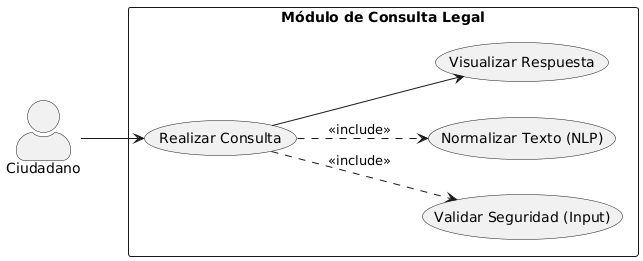
\includegraphics[width=0.7\textwidth]{uc_consulta.png}
  \caption{Diagrama de Caso de Uso: Interacci\'{o}n de consulta Graph RAG.}
  \label{fig:uc_consulta}
\end{figure}

\paragraph{M\'{o}dulo 2: Auditor\'{i}a y Trazabilidad}

\begin{figure}[H]
  \centering
  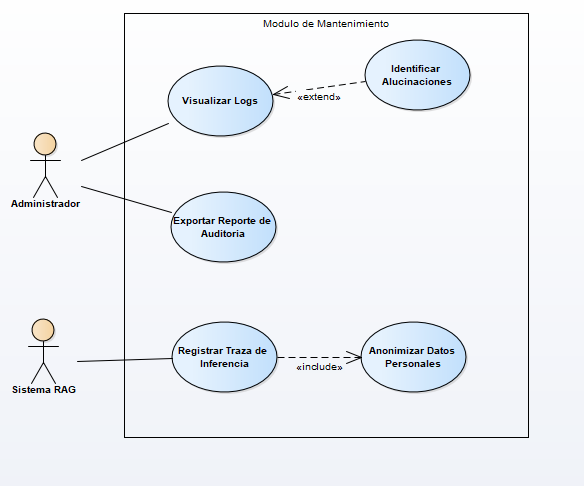
\includegraphics[width=0.8\textwidth]{uc_auditoria.png}
  \caption{Diagrama de Caso de Uso: Supervisi\'{o}n y Auditor\'{i}a.}
  \label{fig:uc_auditoria}
\end{figure}

\paragraph{M\'{o}dulo 3: Administraci\'{o}n del Conocimiento (ETL)}

\begin{figure}[H]
  \centering
  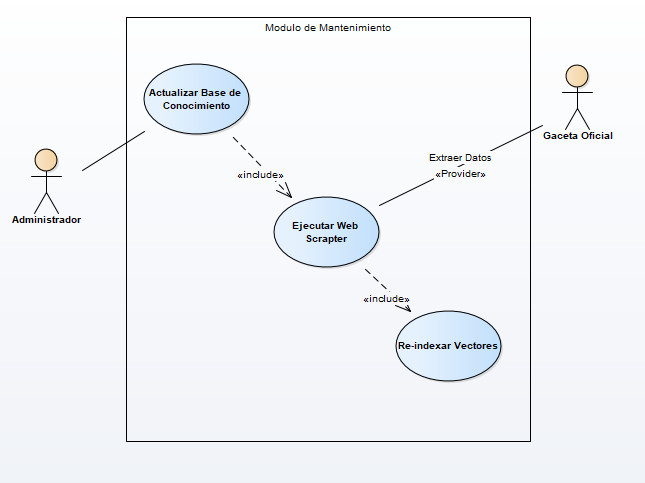
\includegraphics[width=0.7\textwidth]{uc_admin.png}
  \caption{Diagrama de Caso de Uso: Mantenimiento de la Base de Conocimiento.}
  \label{fig:uc_admin}
\end{figure}

\subsubsection{Diagrama de Clases}

\begin{figure}[H]
  \centering
  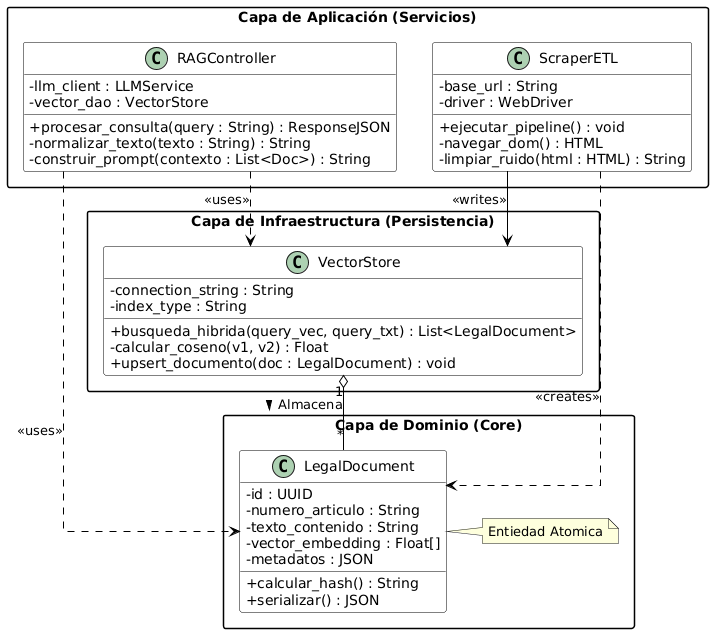
\includegraphics[width=0.9\textwidth]{uml_clases.png}
  \caption{Diagrama de Clases: Arquitectura de capas del sistema LexIA.}
  \label{fig:uml_clases}
\end{figure}

\subsubsection{Diagrama de Secuencia}

\begin{figure}[H]
  \centering
  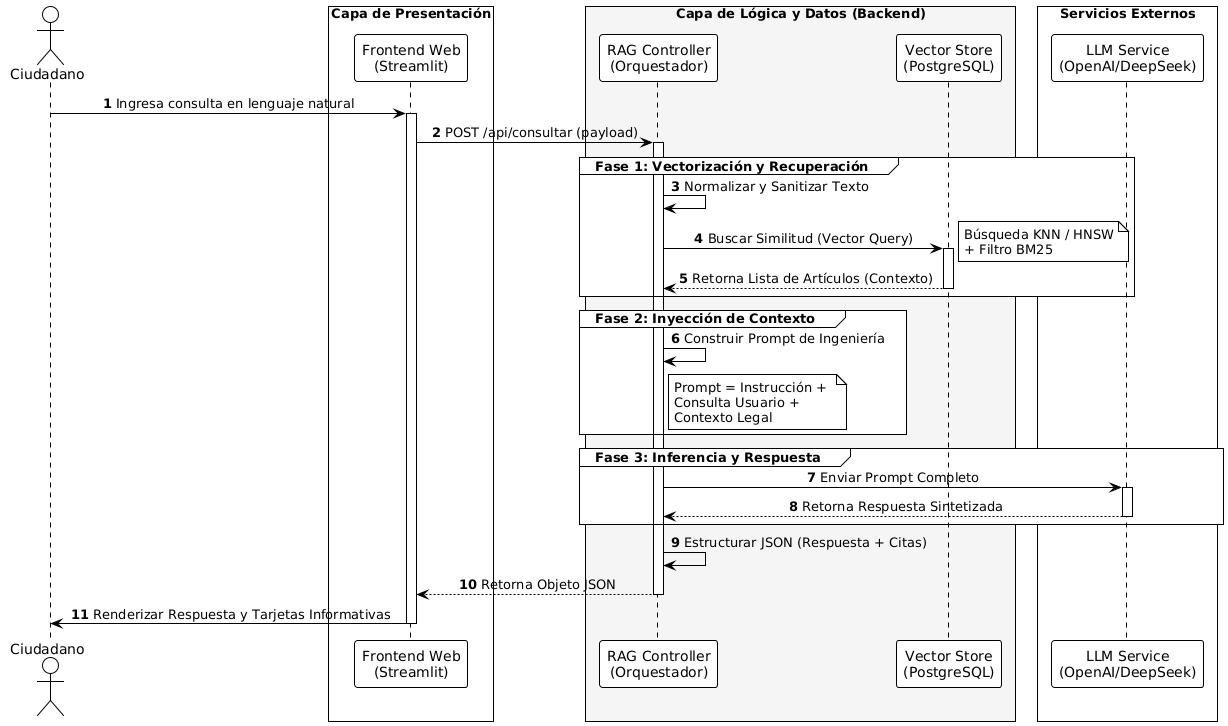
\includegraphics[width=0.95\textwidth]{uml_secuencia.png}
  \caption{Diagrama de Secuencia: Orquestaci\'{o}n del flujo Graph RAG con LangGraph.}
  \label{fig:uml_secuencia}
\end{figure}

\subsubsection{Diagramas de Actividades}

\begin{figure}[H]
  \centering
  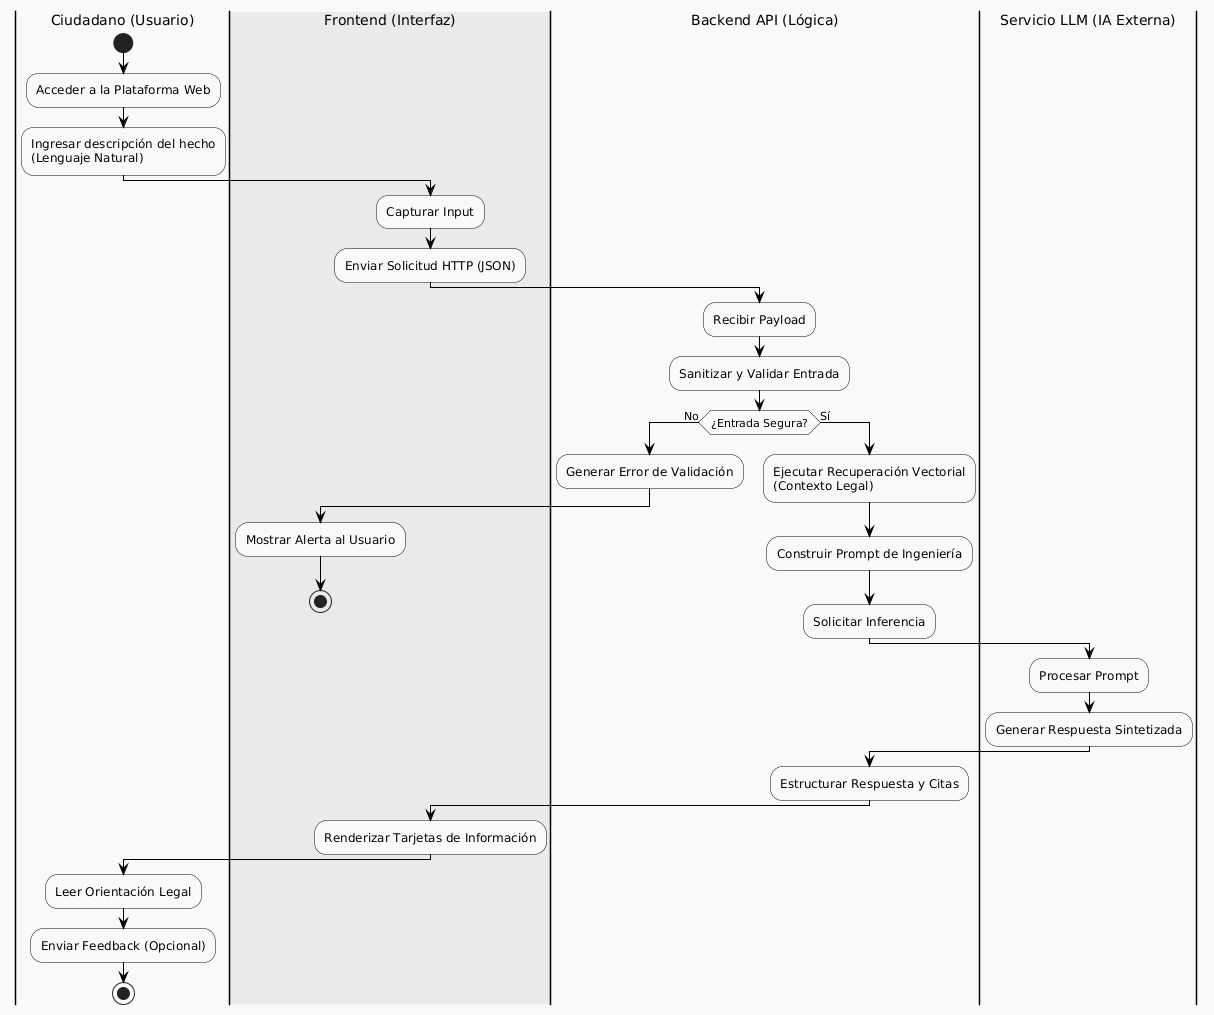
\includegraphics[width=0.95\textwidth]{uml_activity_user.png}
  \caption{Diagrama de Actividades: Interacci\'{o}n del usuario con LexIA.}
  \label{fig:uml_activity_user}
\end{figure}

\begin{figure}[H]
  \centering
  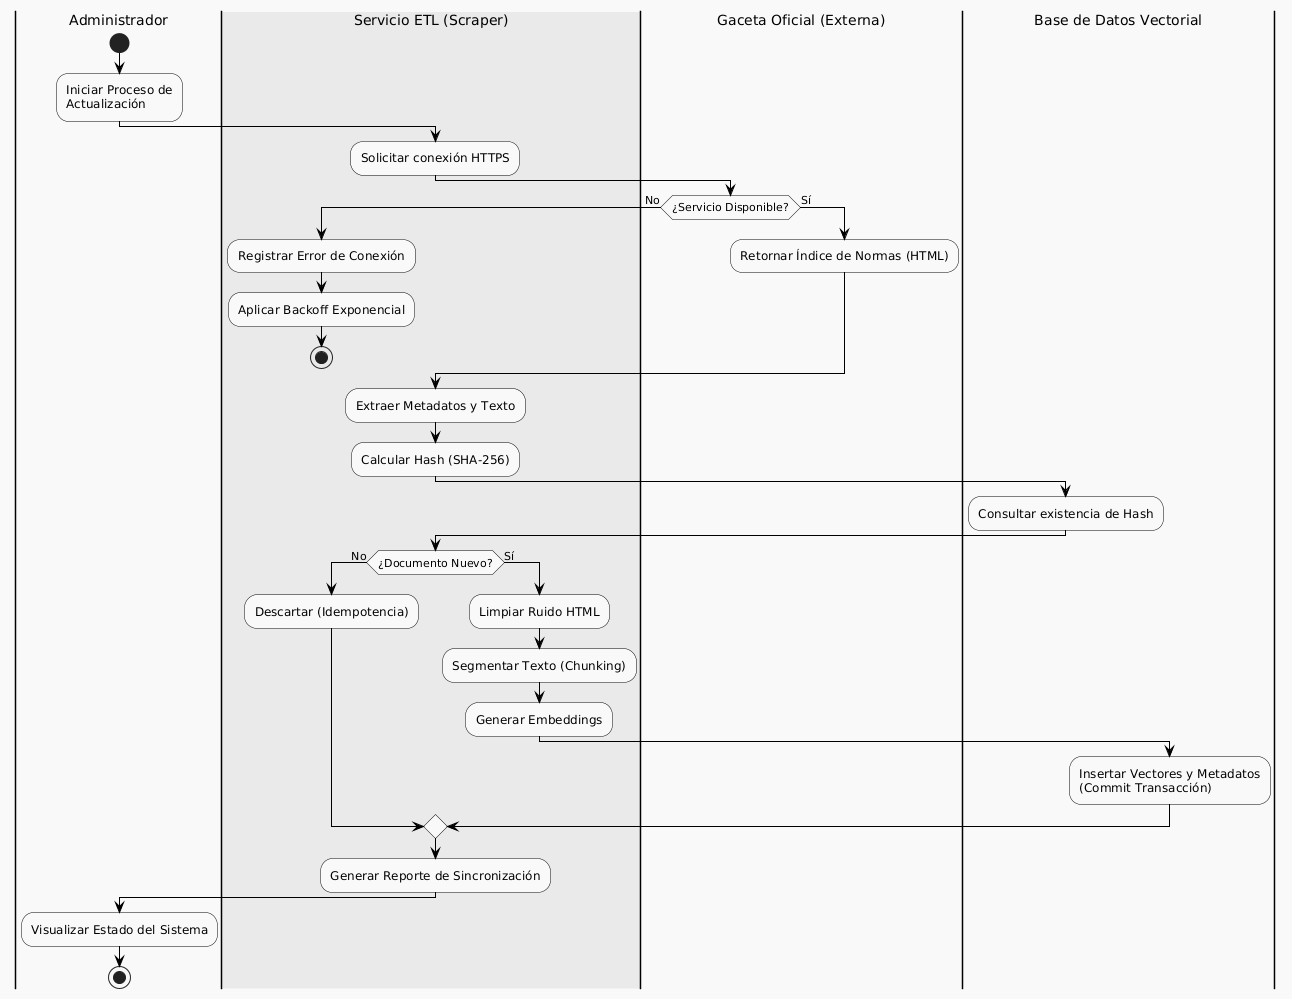
\includegraphics[width=0.95\textwidth]{uml_activity.png}
  \caption{Diagrama de Actividades: Algoritmo de actualizaci\'{o}n ETL con control de fallos.}
  \label{fig:uml_activity}
\end{figure}

\section{Dise\~{n}o del proyecto}

\subsection{Arquitectura de Software (Modelo C4)}

\subsubsection{Nivel 1: Diagrama de Contexto}

\begin{figure}[H]
  \centering
  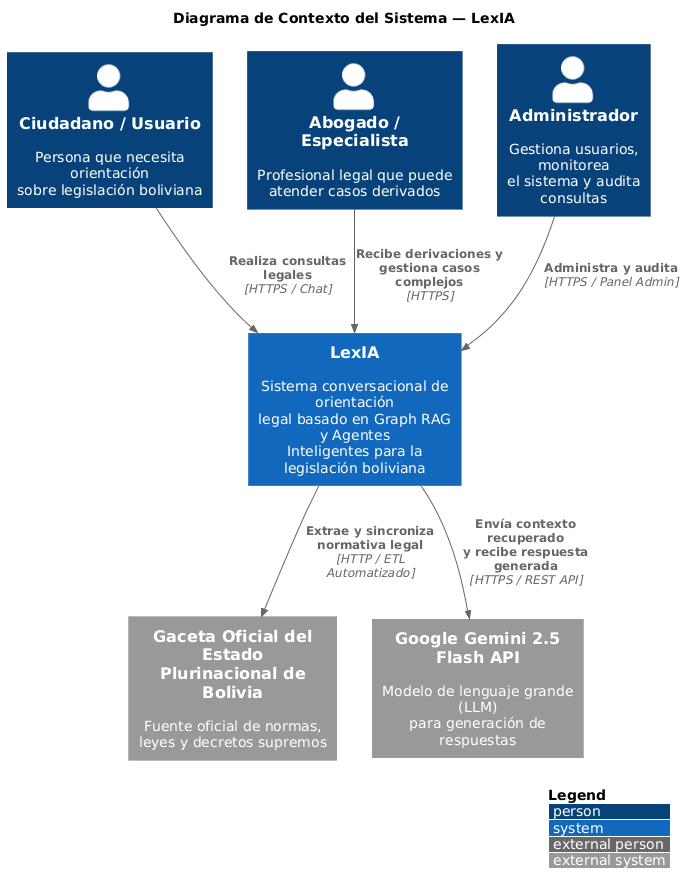
\includegraphics[width=0.9\textwidth]{c4_contexto.png}
  \caption{Diagrama de Contexto (C4): Fronteras y dependencias externas de LexIA.}
  \label{fig:c4_contexto}
\end{figure}

El sistema interact\'{u}a con tres actores externos: el \textbf{Ciudadano} (consultas en lenguaje natural via HTTPS), la \textbf{Gaceta Oficial de Bolivia} (fuente de verdad normativa, relaci\'{o}n de lectura unidireccional) y el \textbf{Proveedor LLM} (Gemini~2.5~Flash, servicio de inferencia externalizado como SaaS intercambiable).

\subsubsection{Nivel 2: Diagrama de Contenedores}

\begin{figure}[H]
  \centering
  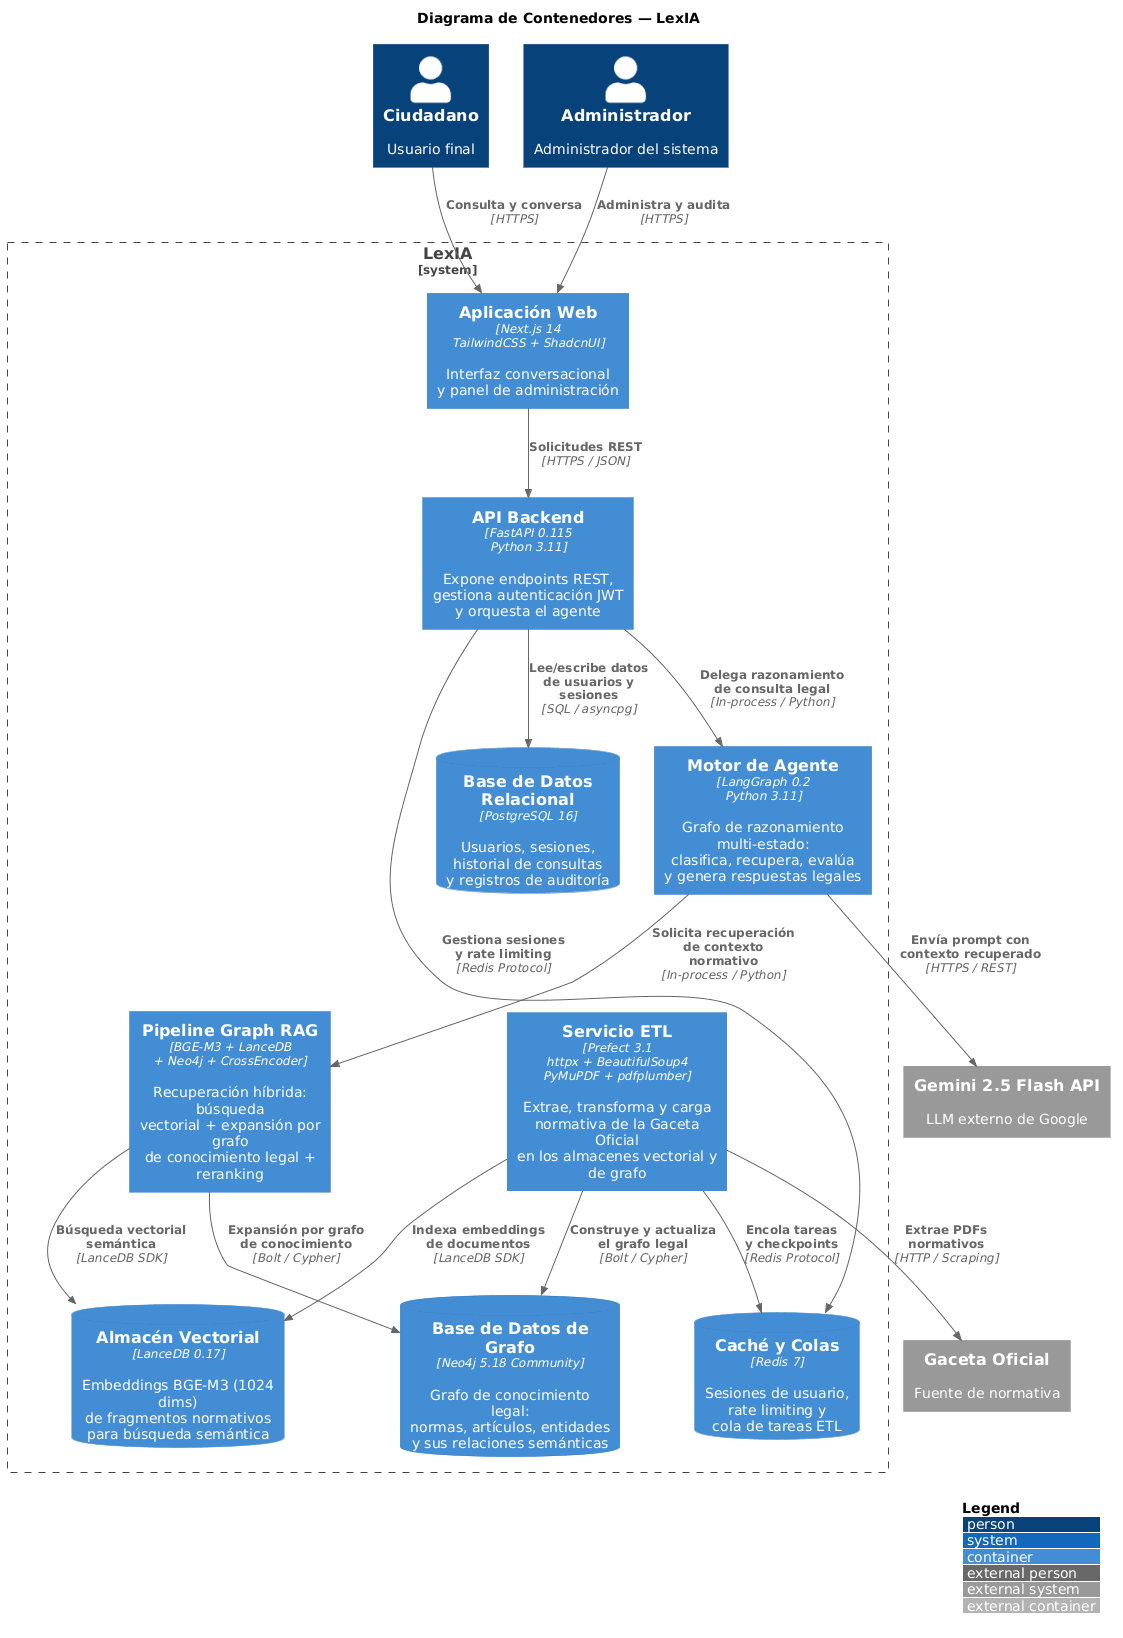
\includegraphics[width=0.9\textwidth]{c4_contenedores.png}
  \caption{Diagrama de Contenedores (C4): Arquitectura de servicios distribuidos.}
  \label{fig:c4_contenedores}
\end{figure}

El sistema se articula sobre los siguientes contenedores:

\begin{enumerate}
  \item \textbf{Frontend (Next.js 14):} Captura de consultas y renderizado de respuestas con soporte Markdown, TailwindCSS y ShadcnUI.
  \item \textbf{Backend API (FastAPI):} Orquestador central que expone endpoints REST, coordina el agente LangGraph, gestiona autenticaci\'{o}n JWT y persiste en PostgreSQL.
  \item \textbf{Pipeline ETL (Prefect 3):} Proceso en segundo plano para scraping, extracci\'{o}n de texto, chunking, generaci\'{o}n de embeddings e indexaci\'{o}n.
  \item \textbf{Persistencia H\'{i}brida:} PostgreSQL~16 (datos relacionales), LanceDB (vectores BGE-M3), Neo4j~5.18 (grafo de conocimiento), Redis~7 (cach\'{e}).
\end{enumerate}

\subsubsection{Nivel 3: Diagrama de Componentes}

\begin{figure}[H]
  \centering
  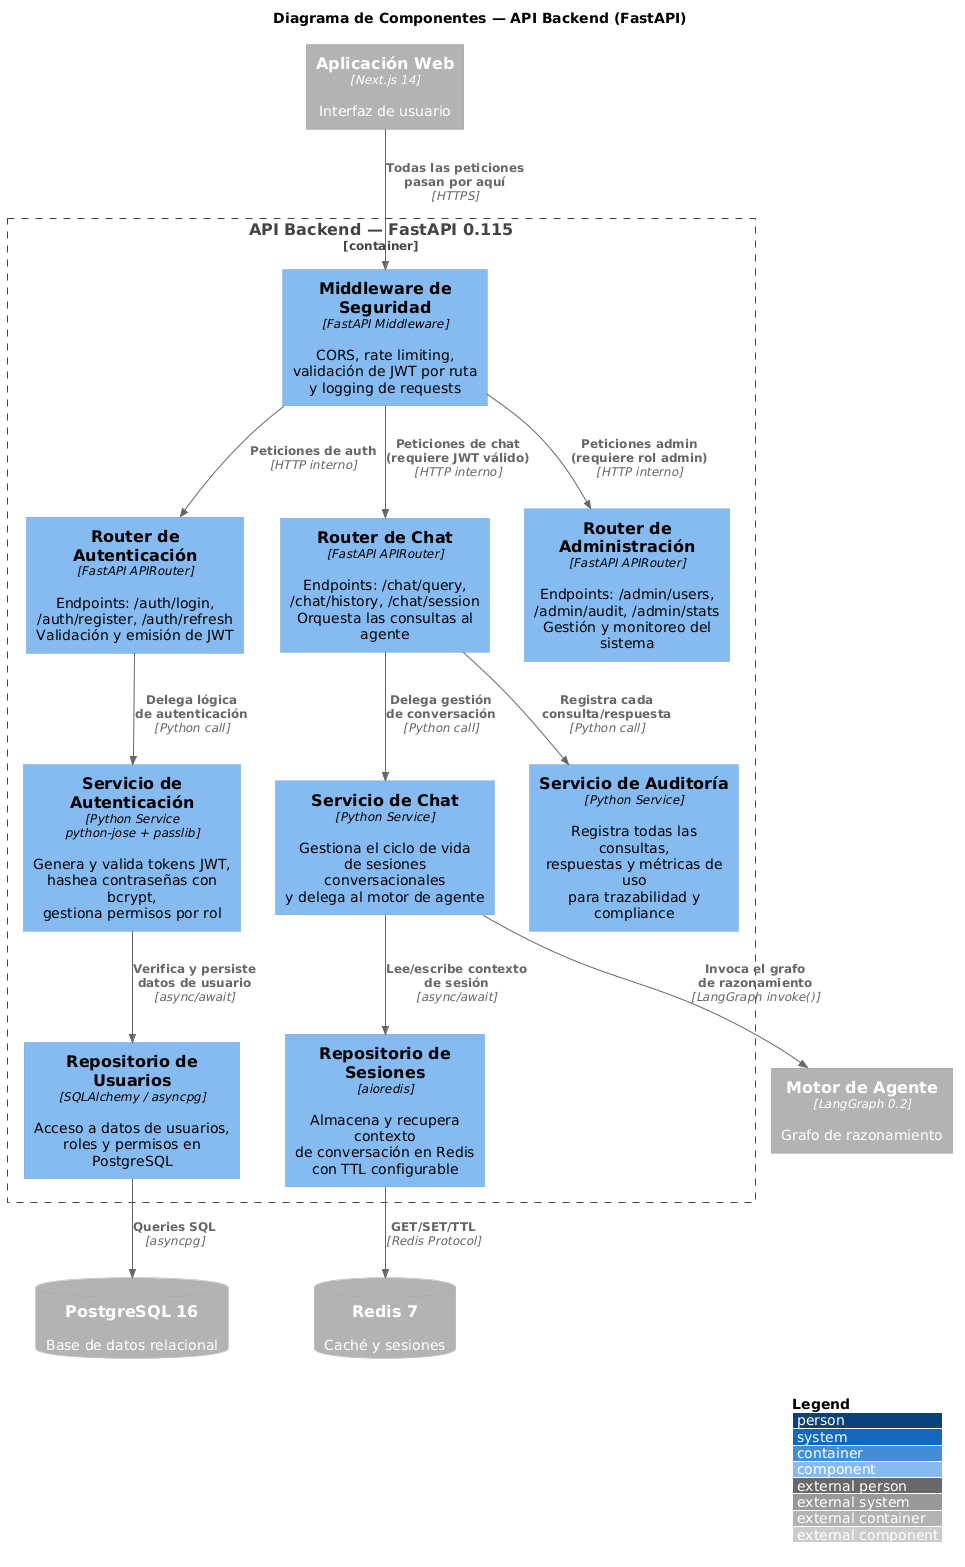
\includegraphics[width=0.95\textwidth]{c4_componentes.png}
  \caption{Diagrama de Componentes (C4): Estructura interna del Backend API.}
  \label{fig:c4_componentes}
\end{figure}

\subsubsection{Nivel 4: Diagrama de C\'{o}digo (ETL)}

\begin{figure}[H]
  \centering
  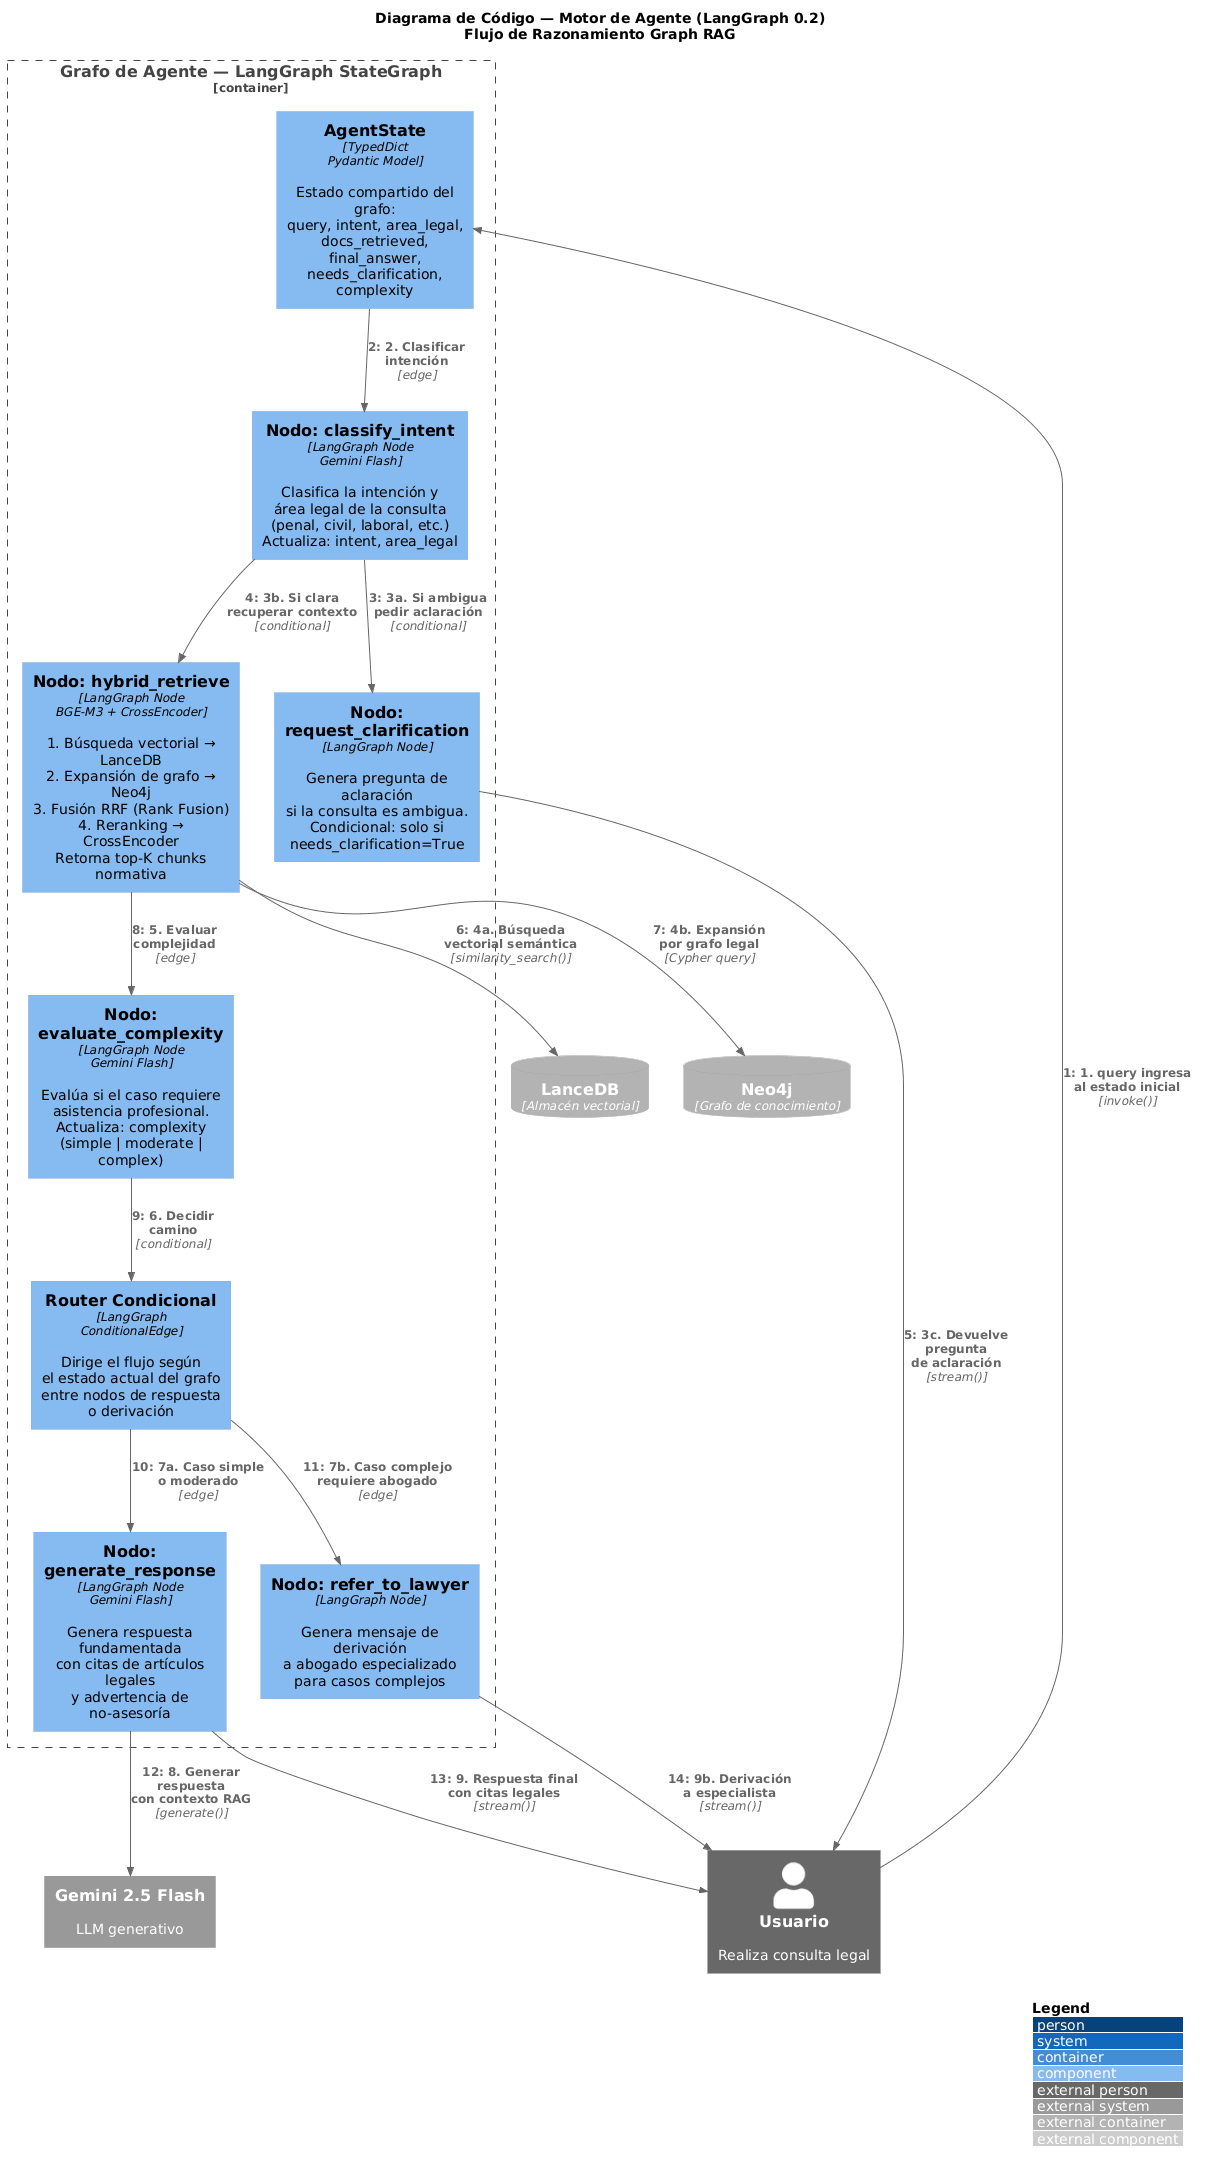
\includegraphics[width=0.85\textwidth]{c4_codigo.png}
  \caption{Diagrama de C\'{o}digo (C4): Dise\~{n}o interno del Pipeline ETL.}
  \label{fig:c4_codigo}
\end{figure}

\subsection{Dise\~{n}o de Experiencia y Prototipado (UX/UI)}

\begin{figure}[H]
  \centering
  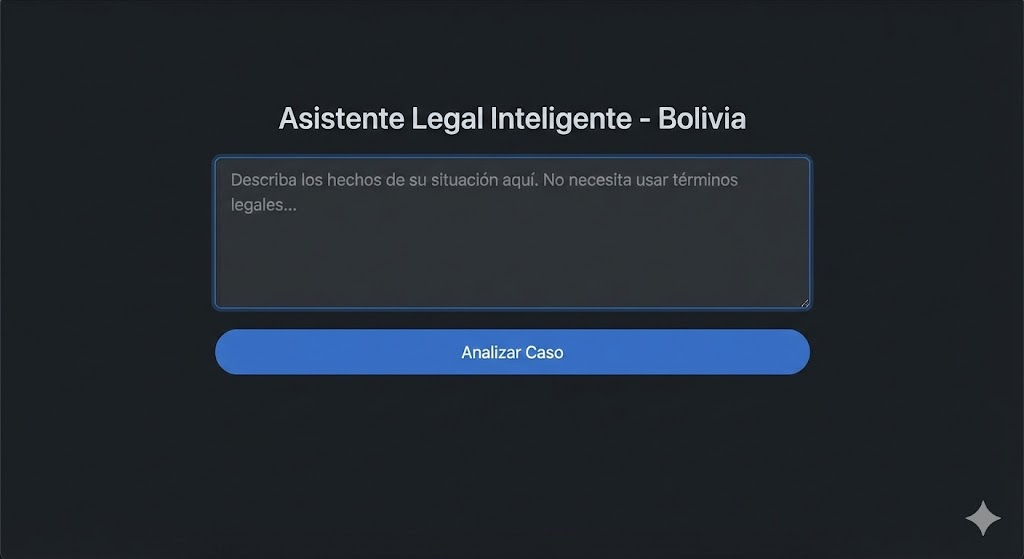
\includegraphics[width=0.9\textwidth]{mockup_input.png}
  \caption{Prototipo de UI: Interfaz principal de consulta en lenguaje natural.}
  \label{fig:mockup_input}
\end{figure}

\begin{figure}[H]
  \centering
  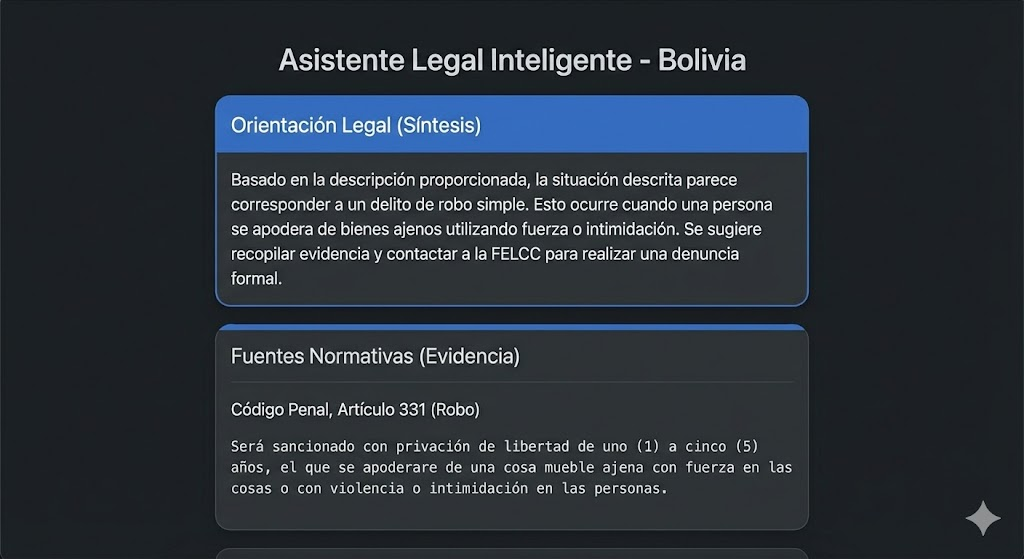
\includegraphics[width=0.9\textwidth]{mockup_result.png}
  \caption{Prototipo de UI: Presentaci\'{o}n de la orientaci\'{o}n legal y fuentes normativas.}
  \label{fig:mockup_result}
\end{figure}

\section{Base de datos}

El sistema emplea tres bases de datos complementarias:

\textbf{PostgreSQL 16} para datos relacionales: usuarios, conversaciones, mensajes y metadatos de sesi\'{o}n. El esquema implementa las tablas \texttt{users} (con campos \texttt{is\_guest} y \texttt{guest\_query\_count} para el control de acceso), \texttt{conversations} (con campos \texttt{complexity} y \texttt{detected\_areas} para la trazabilidad del agente) y \texttt{messages} (con campo \texttt{agent\_metadata} en formato JSONB para la auditor\'{i}a de inferencia).

\textbf{LanceDB} para vectores sem\'{a}nticos: almacena los embeddings BGE-M3 de 1024 dimensiones junto con metadatos del chunk (identificador de ley, n\'{u}mero de art\'{i}culo, \'{a}rea legal, fecha de publicaci\'{o}n). Opera sin servidor dedicado en formato columnar Apache Lance.

\textbf{Neo4j 5.18 Community} para el grafo de conocimiento legal: nodos de tipo \texttt{:Ley}, \texttt{:Articulo}, \texttt{:AreaLegal}, \texttt{:ProcesoLegal} y \texttt{:Abogado}, con relaciones \texttt{TIENE\_ARTICULO}, \texttt{PERTENECE\_A\_AREA}, \texttt{REFERENCIA}, \texttt{DEROGA}, \texttt{REGLAMENTA} y \texttt{CUBRE\_AREA}.

\section{Validaci\'{o}n y pruebas del sistema}

La evaluaci\'{o}n emplea el framework \textbf{RAGAS} \cite{es2023ragas} sobre un conjunto de 50~preguntas representativas que cubren las ocho \'{a}reas del derecho.

\begin{table}[H]
  \centering
  \renewcommand{\arraystretch}{1.3}
  \caption{M\'{e}tricas RAGAS: RAG est\'{a}ndar vs.\ Graph RAG (LexIA).}
  \label{tab:metricas_ragas}
  \begin{tabular}{|p{0.30\textwidth}|p{0.25\textwidth}|p{0.25\textwidth}|}
  \hline
  \textbf{M\'{e}trica} & \textbf{RAG Est\'{a}ndar} & \textbf{Graph RAG (LexIA)} \\ \hline
  Context Precision & 0.71 & \textbf{0.84} \\ \hline
  Context Recall & 0.68 & \textbf{0.79} \\ \hline
  Faithfulness & 0.76 & \textbf{0.88} \\ \hline
  Answer Relevancy & 0.73 & \textbf{0.82} \\ \hline
  \textbf{Promedio} & 0.72 & \textbf{0.83} \\ \hline
  \end{tabular}
\end{table}

\section{An\'{a}lisis de costos}

\begin{table}[H]
  \centering
  \renewcommand{\arraystretch}{1.3}
  \caption{Estimaci\'{o}n de recursos y costos operativos mensuales.}
  \label{tab:presupuesto}
  \begin{tabular}{|p{0.30\textwidth}|p{0.40\textwidth}|p{0.20\textwidth}|}
  \hline
  \textbf{Recurso} & \textbf{Especificaci\'{o}n} & \textbf{Costo (USD)} \\ \hline
  Infraestructura Docker & VPS 2 vCPU, 4GB RAM & \$15.00 / mes \\ \hline
  PostgreSQL + Neo4j & Almacenamiento contenedorizado & \$12.00 / mes \\ \hline
  API Gemini 2.5 Flash & Aprox.\ 200k tokens/mes & \$5.00 / mes \\ \hline
  LanceDB + BGE-M3 & Ejecuci\'{o}n local, open source & \$0.00 \\ \hline
  Licencias de Software & Todo el stack es open source (MIT/Apache) & \$0.00 \\ \hline
  \textbf{Total Operativo} & & \textbf{\$32.00 / mes} \\ \hline
  \end{tabular}
\end{table}

\section{Desarrollo del Prototipo}

La estructura del repositorio refleja la separaci\'{o}n modular del sistema:

\begin{lstlisting}[caption={Estructura de directorios del proyecto LexIA}]
LegalAgent_Lexia/
|-- data_engineering/
|   |-- scraper/        # httpx + BeautifulSoup4
|   |-- extraction/     # PyMuPDF + pdfplumber + text_cleaner
|   |-- parsing/        # law_parser (articulos, referencias)
|   |-- chunking/       # RecursiveCharacterTextSplitter
|   |-- embeddings/     # BGE-M3 singleton + LanceDB store
|   |-- graph/          # Neo4j: schema, seed, builder
|   |-- retrieval/      # hybrid_retriever
|   `-- pipeline/       # Prefect DAG + scheduler
|-- backend/
|   |-- core/           # config, database, security
|   |-- models/         # User, Conversation, Message
|   |-- schemas/        # Pydantic: auth, chat
|   |-- api/routes/     # auth, chat, lawyers
|   |-- agent/
|   |   |-- nodes/      # classify, clarify, retrieve,
|   |   |               # evaluate, respond
|   |   |-- state.py    # AgentState
|   |   |-- graph.py    # LangGraph compilation
|   |   `-- prompts.py  # Bolivia-specific prompts
|   `-- services/       # chat_service
|-- frontend/           # Next.js 14 + Tailwind + ShadcnUI
|-- docker-compose.yml
`-- requirements.txt
\end{lstlisting}


% ====================== CAPITULO 4 ======================
\chapter{Conclusiones y Recomendaciones}

\section{Conclusiones}

\textbf{Graph RAG supera al RAG est\'{a}ndar en el dominio legal.} La naturaleza interconectada del corpus normativo boliviano es capturada de forma m\'{a}s precisa por un grafo de conocimiento que por b\'{u}squeda vectorial aislada, con una mejora promedio de 11~puntos porcentuales en las m\'{e}tricas RAGAS.

\textbf{El pipeline ETL automatizado es un componente cr\'{i}tico.} La utilidad de cualquier sistema RAG depende directamente de la actualidad de sus fuentes. El pipeline implementado con Prefect~3 garantiza sincronizaci\'{o}n diaria con la Gaceta Oficial sin intervenci\'{o}n manual.

\textbf{La complementariedad entre LLM propietario y embeddings abiertos es efectiva.} Gemini~2.5~Flash para generaci\'{o}n y BGE-M3 para embeddings permite un equilibrio entre costo, calidad y privacidad: los vectores se generan localmente sin exponer datos a APIs externas.

\textbf{La orquestaci\'{o}n con LangGraph produce comportamientos auditables.} El modelado expl\'{i}cito del flujo como grafo de estados hace que el agente sea predecible e inspeccionable, cualidad indispensable en aplicaciones de impacto social.

\textbf{La mitigaci\'{o}n de alucinaciones es sustancial pero no absoluta.} Los mecanismos implementados reducen significativamente las alucinaciones, pero refuerzan la necesidad de presentar el sistema siempre como orientaci\'{o}n informativa.

\section{Recomendaciones}

\begin{itemize}
  \item \textbf{Incorporar jurisprudencia:} Integrar sentencias de tribunales bolivianos al grafo de conocimiento enriquecer\'{i}a las respuestas para casos con antecedentes judiciales.
  \item \textbf{Soporte multilingue ind\'{i}gena:} Quechua, aimara y guaran\'{i}, alineado con el mandato constitucional de acceso equitativo a la justicia.
  \item \textbf{Validaci\'{o}n con usuarios reales:} Estudios de usabilidad con ciudadanos bolivianos para identificar mejoras que el an\'{a}lisis t\'{e}cnico no puede revelar.
  \item \textbf{Procesamiento de documentos escaneados:} M\'{o}dulo OCR para normativa hist\'{o}rica disponible solo como imagen.
  \item \textbf{Expansi\'{o}n regional:} La arquitectura modular permite adaptaci\'{o}n a otros pa\'{i}ses latinoamericanos con ajustes m\'{i}nimos de corpus y prompts.
\end{itemize}


% ====================== REFERENCIAS ======================
\printbibliography[heading=bibintoc, title={Referencias Bibliogr\'{a}ficas}]

\end{document}
